\documentclass[a4paper]{article}
\usepackage{graphicx}
\usepackage{amsmath, amsfonts, geometry, float, listings, enumerate, multicol}
\usepackage{multicol, float, colortbl}
\usepackage{lipsum}
\usepackage{tikz, titlesec, parskip}
\usepackage{tikz,pgfplots, circuitikz}
\usepackage{epsfig,graphicx,amsthm,amsmath}
\usepackage{wrapfig}
\usepackage{subfigure}
\usepackage{caption}
\usepackage{subfigure}
\usepackage{graphicx}
\usepackage{pythontex} 
\usepackage{matlab-prettifier}
\usepackage{tabularx}
\usepackage{media9}
\usepackage[utf8]{inputenc}
\usepackage{color}

\usepackage{caption, enumitem}
\definecolor{forest}{RGB}{34,139,34}
\definecolor{c1}{RGB}{0,128,255}
\definecolor{c2}{RGB}{0,204,102}
\definecolor{c3}{RGB}{0,128,128}
\definecolor{c4}{RGB}{255,102,102}
\definecolor{c5}{RGB}{130,50,220}
\definecolor{c6}{RGB}{0,204,102}
\definecolor{c7}{RGB}{255,153,51}
\definecolor{c8}{RGB}{153,153,255}
\definecolor{c9}{RGB}{160,160,160}
\definecolor{c0}{RGB}{240,200,0}
\usetikzlibrary{arrows,calc,positioning}
\tikzset{
	block/.style = {draw, rectangle,
		minimum height=1cm,
		minimum width=2cm},
	input/.style = {coordinate,node distance=1cm},
	output/.style = {coordinate,node distance=4cm},
	arrow/.style={draw, -latex,node distance=2cm},
	pinstyle/.style = {pin edge={latex-, black,node distance=2cm}},
	sum/.style = {draw, circle, node distance=1cm},
}

\usepackage{relsize}
\usepackage[pagebackref=false,colorlinks,linkcolor=forest,urlcolor= blue,citecolor=blue]{hyperref}

\titlespacing{\section}{0pt}{10pt}{0pt}
\titlespacing{\subsection}{0pt}{10pt}{0pt}
\titlespacing{\subsubsection}{0pt}{10pt}{0pt}

\usetikzlibrary{calc,patterns,through}
\newcommand{\arcangle}{%
	\mathord{<\mspace{-9mu}\mathrel{)}\mspace{2mu}}%
}

\newcommand{\Cross}{$\mathbin{\tikz [x=1.4ex,y=1.4ex,line width=.2ex] \draw (0,0) -- (1,1) (0,1) -- (1,0);}$}%


\renewcommand{\baselinestretch}{1.2}
\geometry{
	a4paper,
	total={170mm,257mm},
	left=20mm,
	top=20mm,
}

\usepackage{hyperref}
\hypersetup{
	colorlinks=true,
	linkcolor=forest,
	filecolor=magenta,      
	urlcolor=cyan,
	pdftitle={Overleaf Example},
	pdfpagemode=FullScreen,
}

\usepackage{fancyhdr}
\pagestyle{fancy}
\fancyhf{}
\rhead{\textbf{ Farzan Aghaei }}
\lhead{\textbf{ Assignment 2 }}
\lfoot{(\space\textbf{\thepage}\space)}
\rfoot{\textbf{Data Networks }}
\renewcommand{\headrulewidth}{1pt}
\renewcommand{\footrulewidth}{1pt}

\renewcommand{\thefootnote}{{footnote}}


\begin{document}
	\begin{minipage}{0.65\textwidth}
		\begin{center}
			\normalsize
			‫		In the name of Allah\\
			\vspace{0.5cm}
			\huge
			\textbf{Data Networks} \\
			\vspace{0.2cm}
			\LARGE
			Prof. Mohammad Reza Pakravan \\
			\vspace{0.5cm}
			\Large
			Assignment 2\\
			\vspace{0.6cm}
			Farzan Aghaei 401101202
			\vspace{0.2cm}
		\end{center}
		\normalsize
	\end{minipage}
	\begin{minipage}{0.35\textwidth}
		\begin{flushleft}
			\centering
			
\includegraphics[width=0.7\textwidth]{Shariflogo.jpg}\\ \large
			
			\vspace{0.4cm}
			Sharif University of Technology\\
			\vspace{0.2cm}
			Electrical Engineering Department\\
			\vspace{0.2cm}
		\end{flushleft}
	\end{minipage}
	
	\rule[0.1\baselineskip]{\textwidth}{1pt}
	
	\section{Performing Measurements Using INET Framework}
	
	\subsection{Measuring Channel Throughput}
	\Large
	a)
	\large
	\begin{center}
		\Large
		$
		\text{Packet Size} = 1200B = 9600 bits\quad
		\text{Arrival Rate} = \dfrac{1}{200\mu s} = 5000 \text{packets per second}\linebreak
		\text{Throughput} = \text{Packet Size} \times \text{Arrival Rate} = 9600 \times 5000 = 48 Mbps
		$
	\end{center}
	
	The channel throughput is 48Mbps based on the given packet size, transmission rate, and production interval.
	
	\begin{figure}[!h]
		\centering
		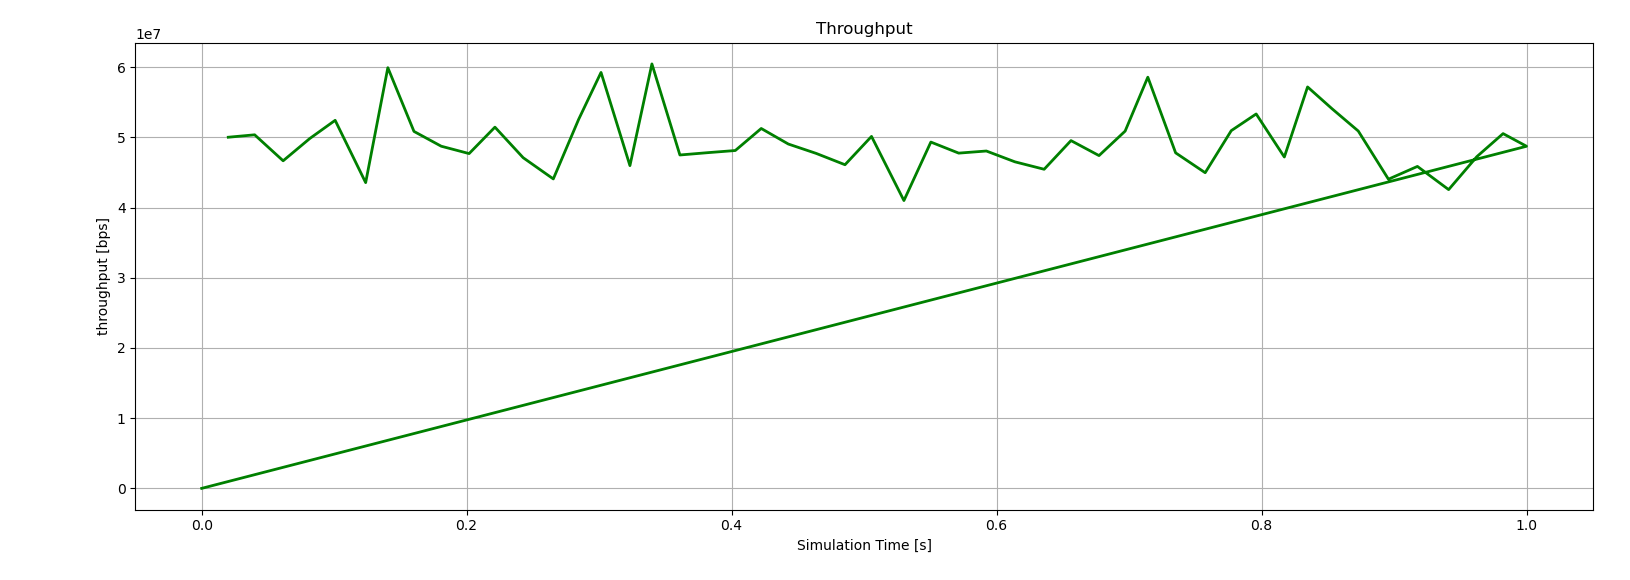
\includegraphics[width=0.8\linewidth]{screenshot001}
		\caption{Throughput using 1200B packet size and 200$\mu$s mean interval}
		\label{fig:screenshot001}
	\end{figure}
	
	The throughput is fluctuating but stays within the range of 40-60Mbps, which indicates that the average throughput is close to the hand-calculated value of 48Mbps, but the simulation is capturing the variability in packet generation due to the random intervals.
	
	The 40-60Mbps range shows that, in some periods, the network can handle a higher packet rate, potentially utilizing more of the available bandwidth, while during other periods, throughput drops slightly due to random packet generation.
	
	\pagebreak
	\Large
	b)
	\large
	
	\begin{center}
		\Large
		$
		\text{Packet Size} = 600B = 4800 bits\linebreak
		\text{Throughput} = \text{Packet Size} \times \text{Arrival Rate} = 4800 \times 5000 = 24 Mbps
		$
	\end{center}
	
	\begin{figure}[!h]
		\centering
		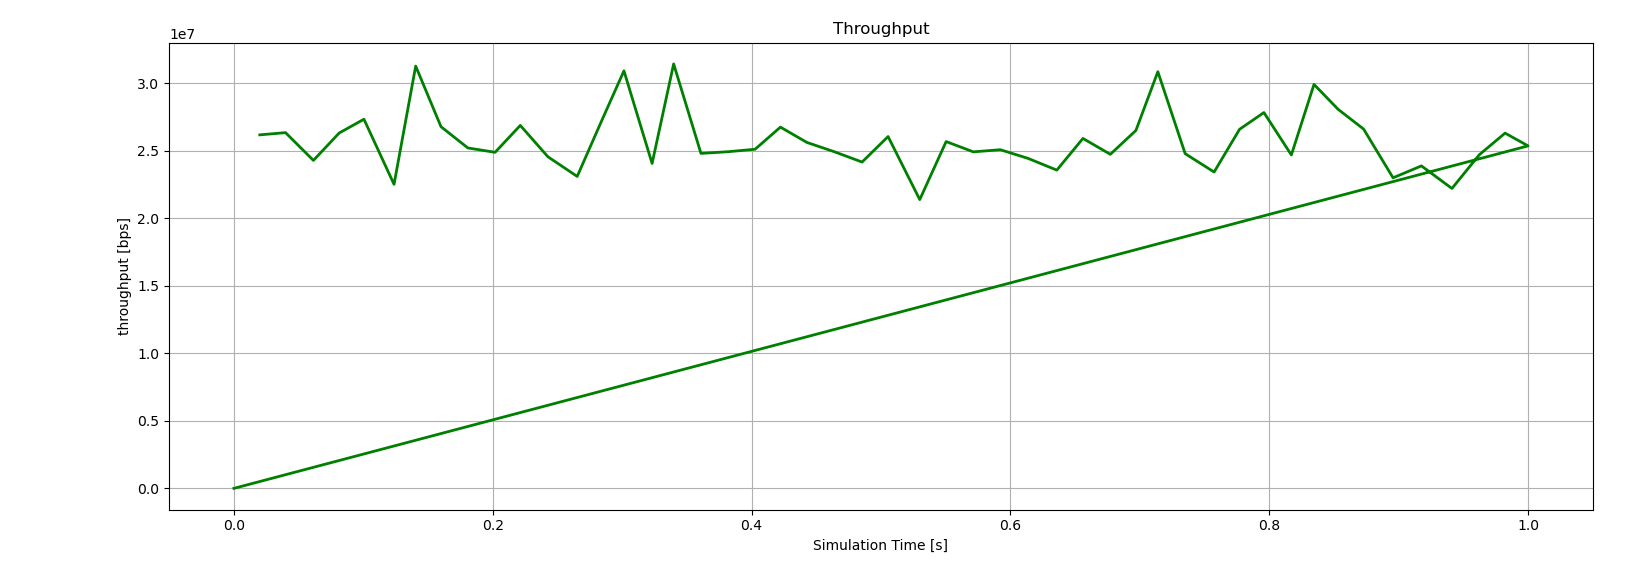
\includegraphics[width=0.8\linewidth]{screenshot002}
		\caption{Throughput using 600B packet size and 200$\mu$s mean interval}
		\label{fig:screenshot002}
	\end{figure}
	
	\begin{center}
		\Large
		$
		\text{Packet Size} = 300B = 2400 bits\linebreak
		\text{Throughput} = \text{Packet Size} \times \text{Arrival Rate} = 2400 \times 5000 = 12 Mbps
		$
	\end{center}
	
	\begin{figure}[!h]
		\centering
		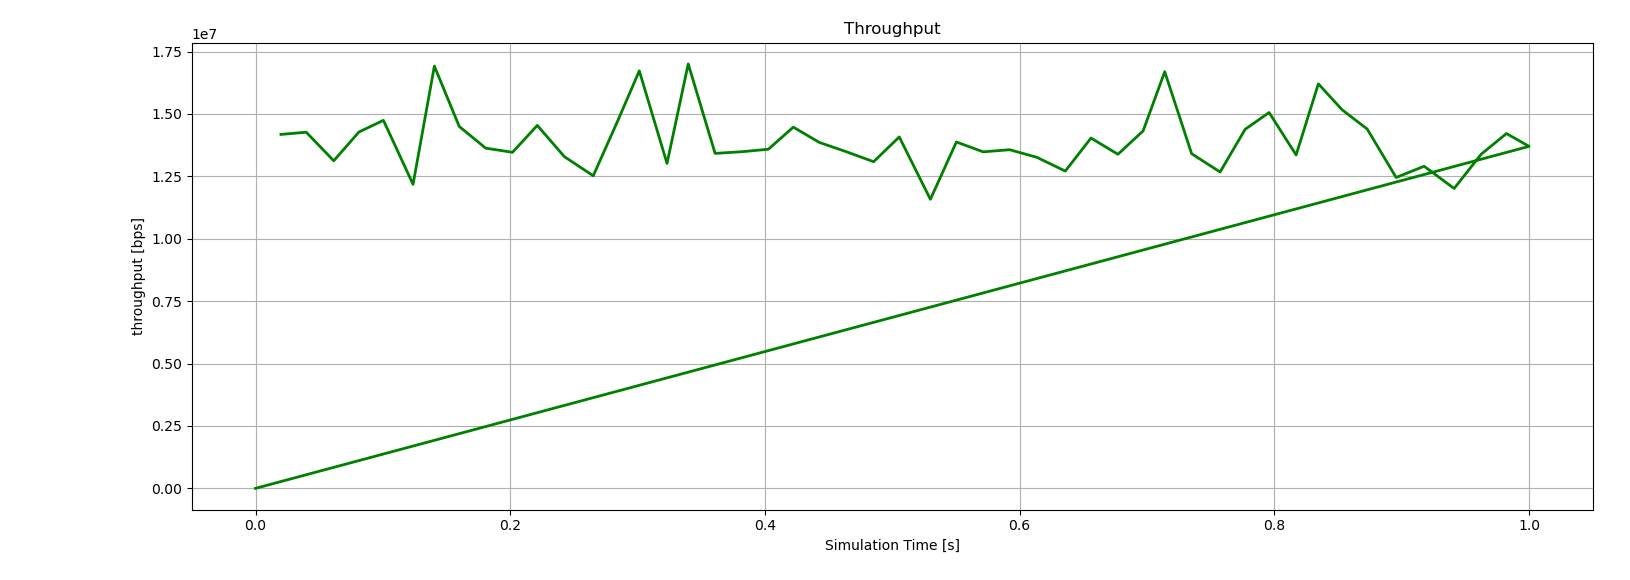
\includegraphics[width=0.8\linewidth]{screenshot003}
		\caption{Throughput using 300B packet size and 200$\mu$s mean interval}
		\label{fig:screenshot003}
	\end{figure}
	
	Throughput decreases as the packet size decreases from 1200B to 600B to 300B, which is expected due to:
	\begin{itemize}
		\item Increased overhead with smaller packets (because the same network overhead is applied to a smaller amount of data).
	
		\item Lower efficiency with smaller packets, as more time is spent transmitting headers and less on actual data transmission.
	\end{itemize}
	The standard deviation decreases as the packet size decreases, indicating less fluctuation in throughput for smaller packets. This may be because the network is underutilized and the variability due to random packet arrival intervals is less pronounced.
	
	1200B packets allow for the highest throughput and efficiency, with a higher standard deviation reflecting the network's attempt to handle larger amounts of data more efficiently but still subject to random variability.
	
	\pagebreak
	
	\Large
	c)
	\large
	\begin{center}
		\Large
		$
		\text{Packet Size} = 1800B = 14400 bits \rightarrow \text{MTU} = 1500B \Rightarrow\linebreak \large\text{a packet larger than 1500-bytes will need to be fragmented into smaller parts.} \Large\rightarrow 1500B + 300B
		\linebreak
		\text{Throughput} = \text{Packet Size} \times \text{Arrival Rate} = 14400 \times 5000 = 72 Mbps
		$
	\end{center}
	
	\begin{figure}[!h]
		\centering
		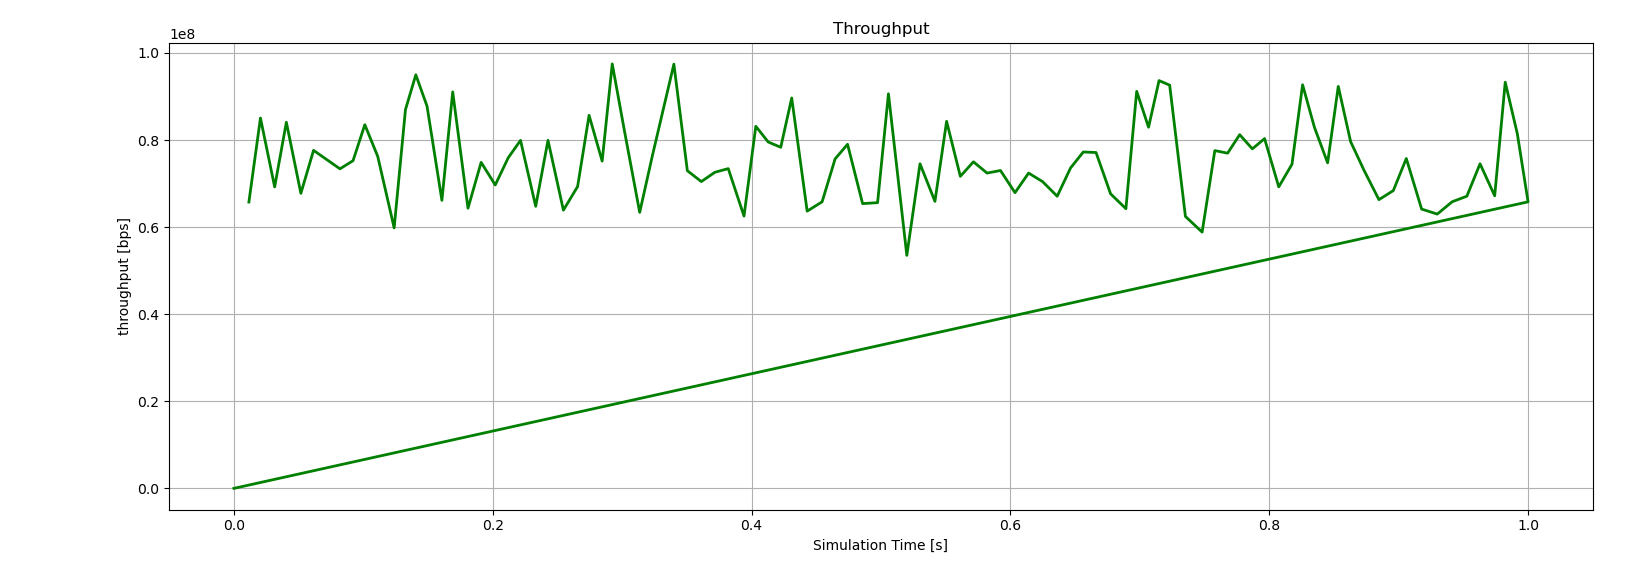
\includegraphics[width=0.8\linewidth]{screenshot004}
		\caption{Throughput using 1800B packet size and 200$\mu$s mean interval}
		\label{fig:screenshot004}
	\end{figure}
	
	Although the Ethernet MTU (Maximum Transmission Unit) is 1500 bytes, the 1800B packets are larger than the MTU, meaning that they must be fragmented into two smaller packets.
	
	Fragmentation increases the number of frames to be transmitted, each requiring its own overhead for headers and processing. This extra overhead causes some fluctuation in throughput, as each fragment of the larger packet is treated separately and can introduce delays, depending on network conditions.
	
	Fragmentation explains why the throughput is not as high as the theoretical maximum, even though the packet size is larger.
	
	The higher mean throughput for 1800B packets is due to larger packets transmitting more data per unit of time, leading to better bandwidth utilization.
	
	The higher deviation reflects the larger fluctuations in throughput, which is caused by:
	\begin{itemize}
		\item Fragmentation (due to the 1800B packet size exceeding the MTU).
	
		\item Increased transmission times and queueing delays.
	
		\item Network congestion or fluctuations in packet processing time.
	\end{itemize}
	Thus, while larger packets lead to better utilization of the link (higher throughput), they also introduce more variability and overhead due to fragmentation and increased transmission time.
	
	\pagebreak
	
	\Large
	d)
	\large
	\begin{center}
		\Large
		$
		\text{Packet Size} = 1200B = 9600 bits\linebreak
		\text{Throughput} = \text{Packet Size} \times \text{Arrival Rate} = 9600 \times 2500 = 24 Mbps
		$
	\end{center}
	
	\begin{figure}[!h]
		\centering
		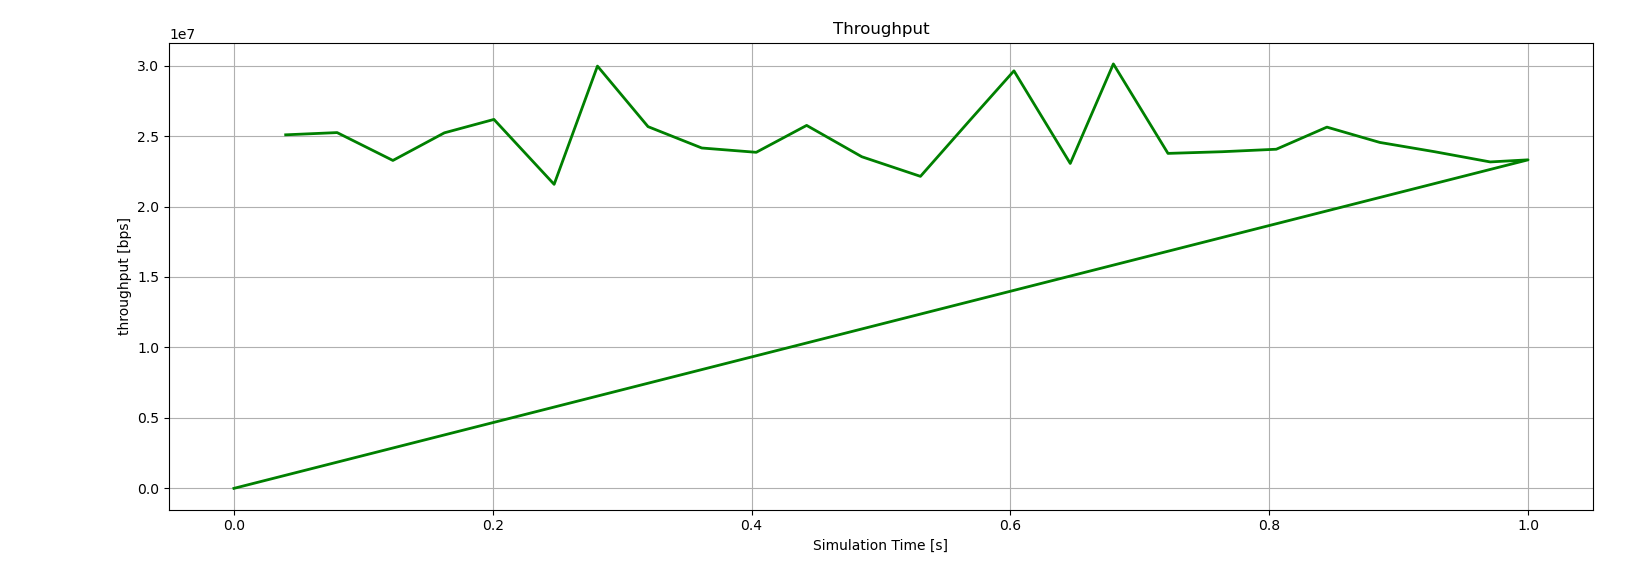
\includegraphics[width=0.8\linewidth]{screenshot005}
		\caption{Throughput using 1200B packet size and 400$\mu$s mean interval}
		\label{fig:screenshot005}
	\end{figure}
	
	The throughput has halved from 48Mbps to 24Mbps due to the reduction in the packet rate caused by increasing the packet generation interval from 200 μs to 400 μs.
	
	The standard deviation has decreased, reflecting less variability in throughput as the network is not being fully utilized. The fluctuations are smaller because the system is operating at a lower average rate and is underutilized.
	
	The random nature of the packet generation still results in fluctuations, but these are now less significant because the packet rate is slower and the network isn't being overloaded with packet arrivals.
	
	\subsection{Measuring Channel Utilization}
	\large
	\begin{center}
		\Large
		$
		\text{Throughput} = 48 Mbps \longrightarrow U = \dfrac{\text{Throughput}}{\text{Channel DataRate}} = \dfrac{48 Mbps}{100 Mbps} = 0.48
		$
	\end{center}
	
	\begin{figure}[!h]
		\centering
		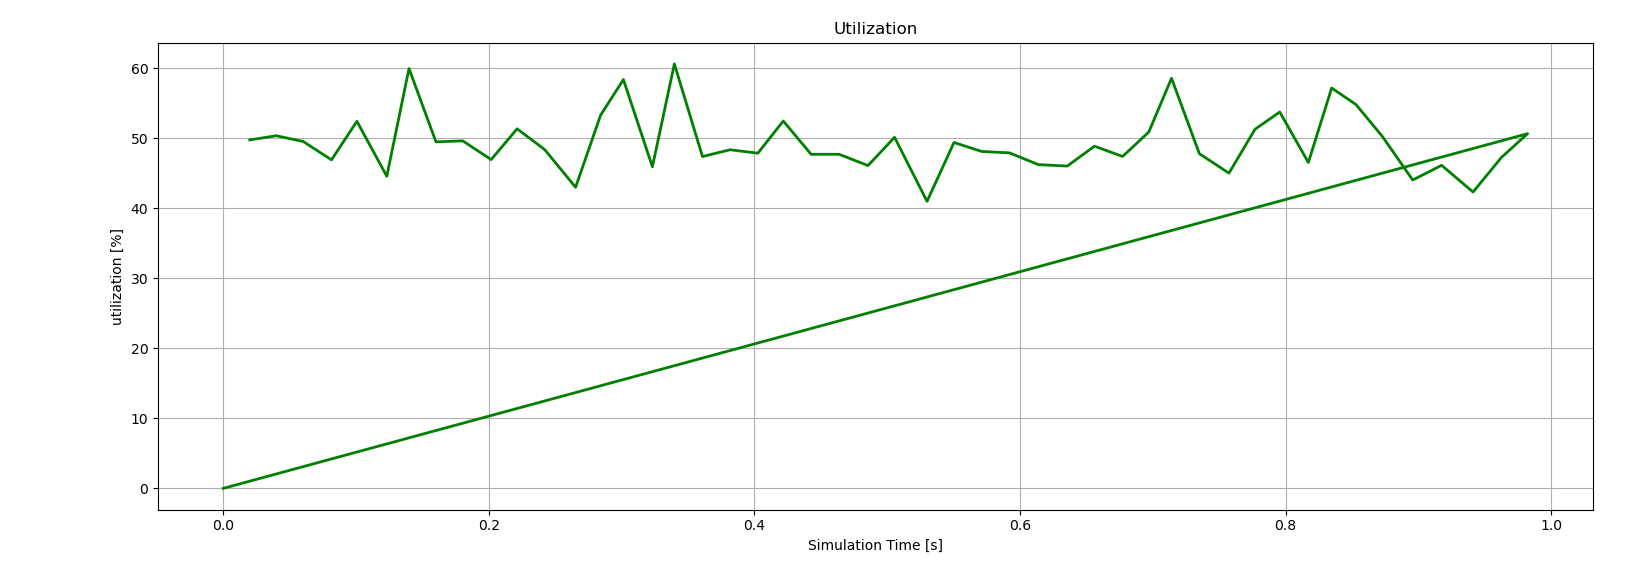
\includegraphics[width=0.8\linewidth]{screenshot006}
		\caption{Utilization}
		\label{fig:screenshot006}
	\end{figure}
	
	The mean utilization of 49.38\% is very close to the calculated value of 48\%, showing that the simulation is accurately modeling the expected network performance.
	
	The deviation of results reflect the randomness of packet generation, where the utilization fluctuates slightly over time.
	The simulation results are consistent with the hand calculations, and the small variations can be attributed to the randomness in packet arrival intervals.
	
	\pagebreak
	
	\subsection{Measuring End-to-end Delay}
	\Large
	a) b)
	\large
	
	\begin{figure}[!h]
		\centering
		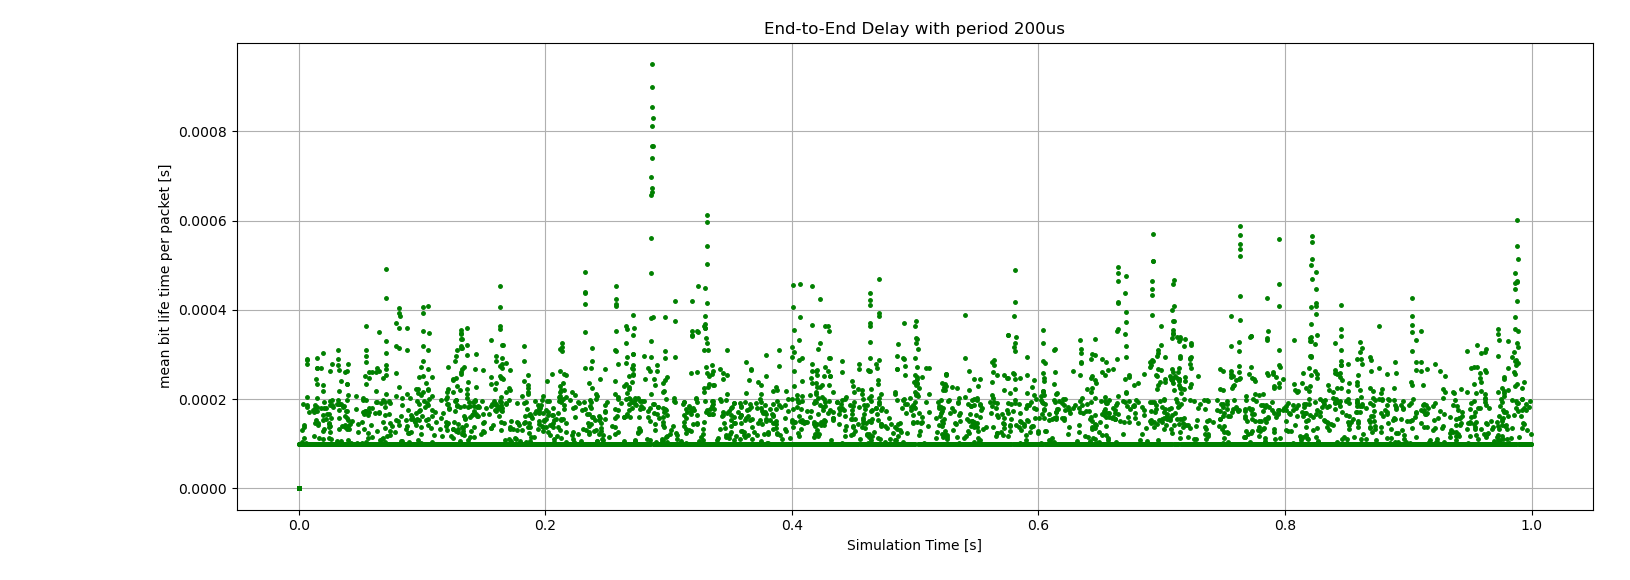
\includegraphics[width=0.75\linewidth]{screenshot007}
		\caption{End-to-End Delay with period 200$\mu$s}
		\label{fig:screenshot007}
	\end{figure}	
	\begin{figure}[!h]
		\centering
		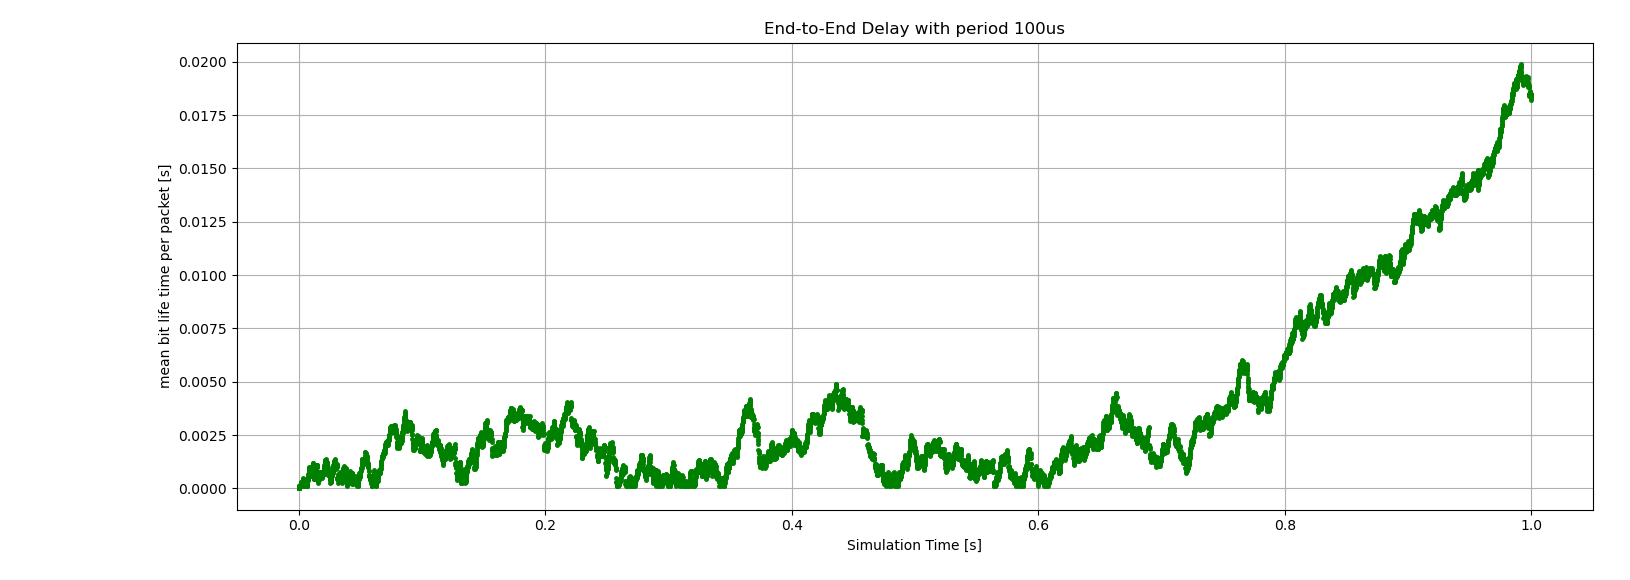
\includegraphics[width=0.75\linewidth]{screenshot009}
		\caption{End-to-End Delay with period 100$\mu$s}
		\label{fig:screenshot009}
	\end{figure}
	
	\begin{figure}[!h]
		\centering
		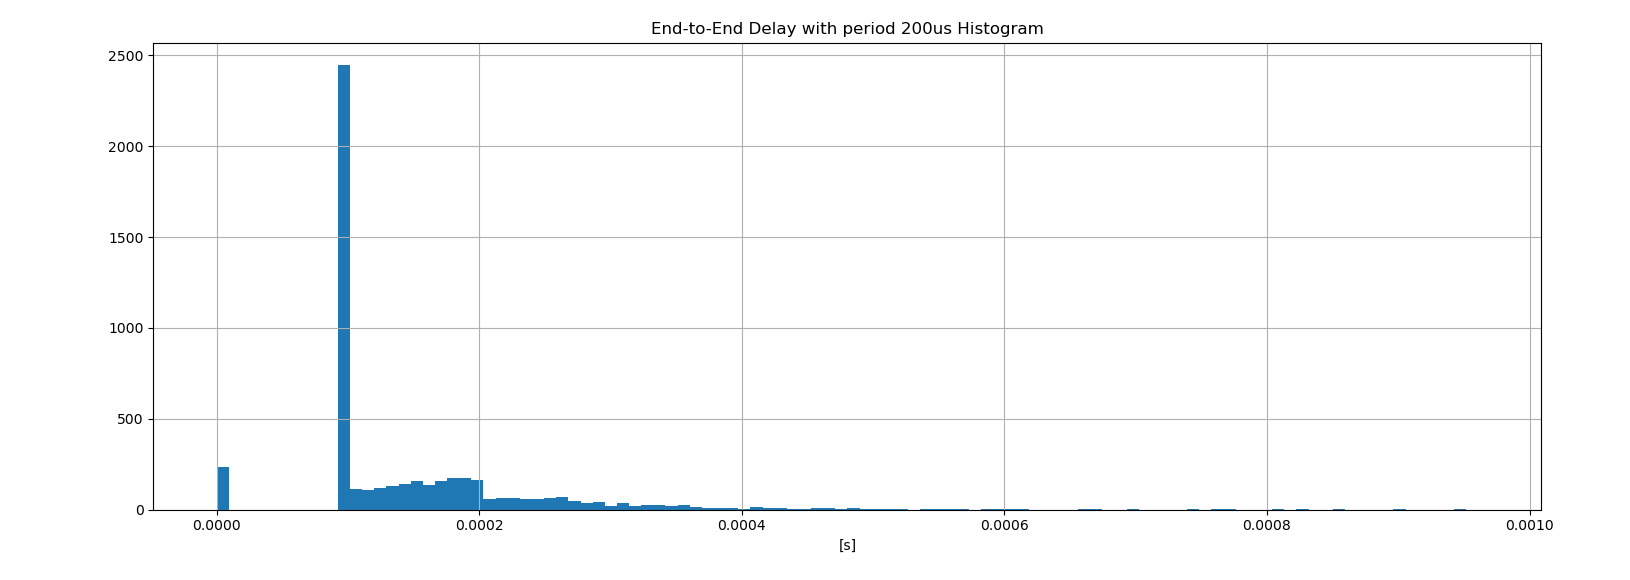
\includegraphics[width=0.75\linewidth]{screenshot008}
		\caption{End-to-End Delay with period 200$\mu$s Histogram}
		\label{fig:screenshot008}
	\end{figure}
	\begin{figure}[!h]
		\centering
		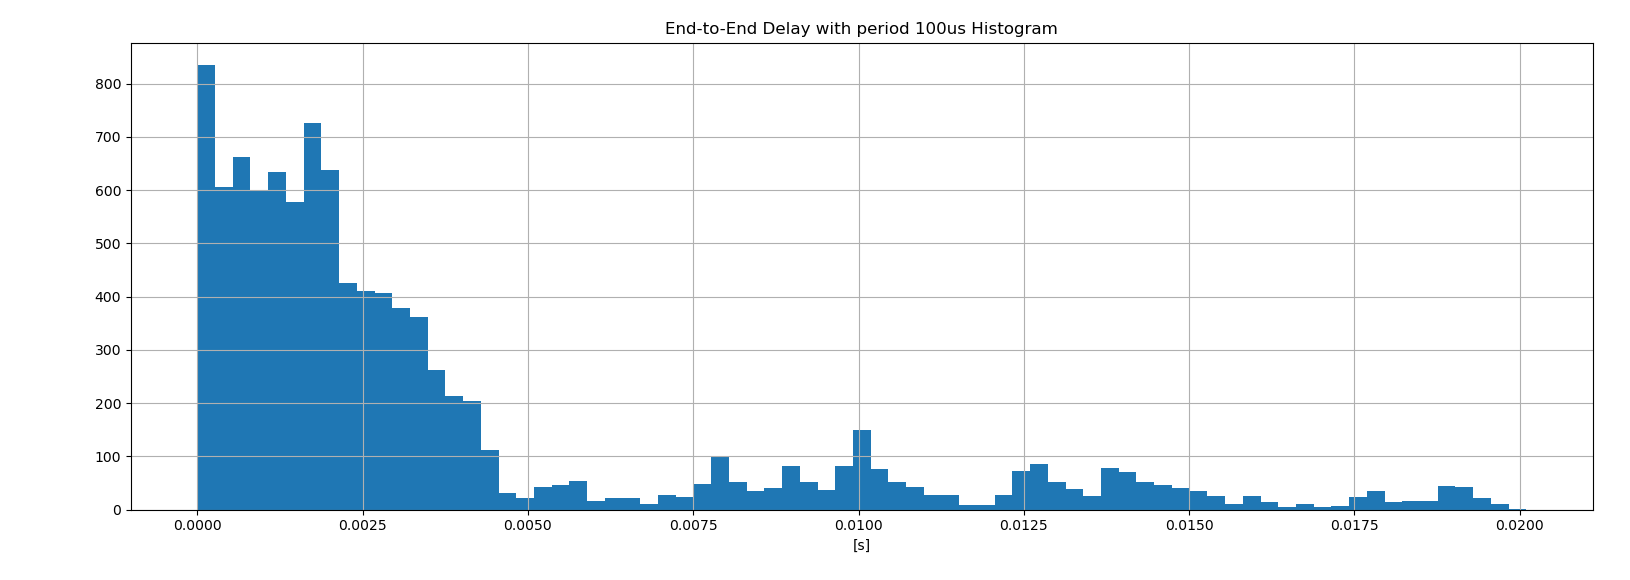
\includegraphics[width=0.75\linewidth]{screenshot010}
		\caption{End-to-End Delay with period 100$\mu$s Histogram}
		\label{fig:screenshot010}
	\end{figure}
	
	\pagebreak
	
	\Large
	c)
	\large
	
	The increase in packet generation rate from 200 μs to 100 μs has caused a significant increase in end-to-end delay, from 153.2 μs to 3.99 ms. This is because the system is now processing packets more frequently, leading to congestion and longer delays.
	
	The higher standard deviation (4.47 ms vs 83.2 μs) for the 100 μs interval indicates that the network is less stable under higher packet arrival rates.
	
	The overall trend shows that faster packet generation leads to higher delay due to increased congestion and processing times.
	
	\subsection{Measuring Transmission Time}
	\large
	\begin{center}
		\Large
		$
		\text{Transmission Time} = \dfrac{\text{Packet Size}}{\text{Channel DataRate}} = \dfrac{\frac{200 + 800}{2}\times8}{100000000} = 40\mu sec
		$
	\end{center}
	
	\begin{figure}[!h]
		\centering
		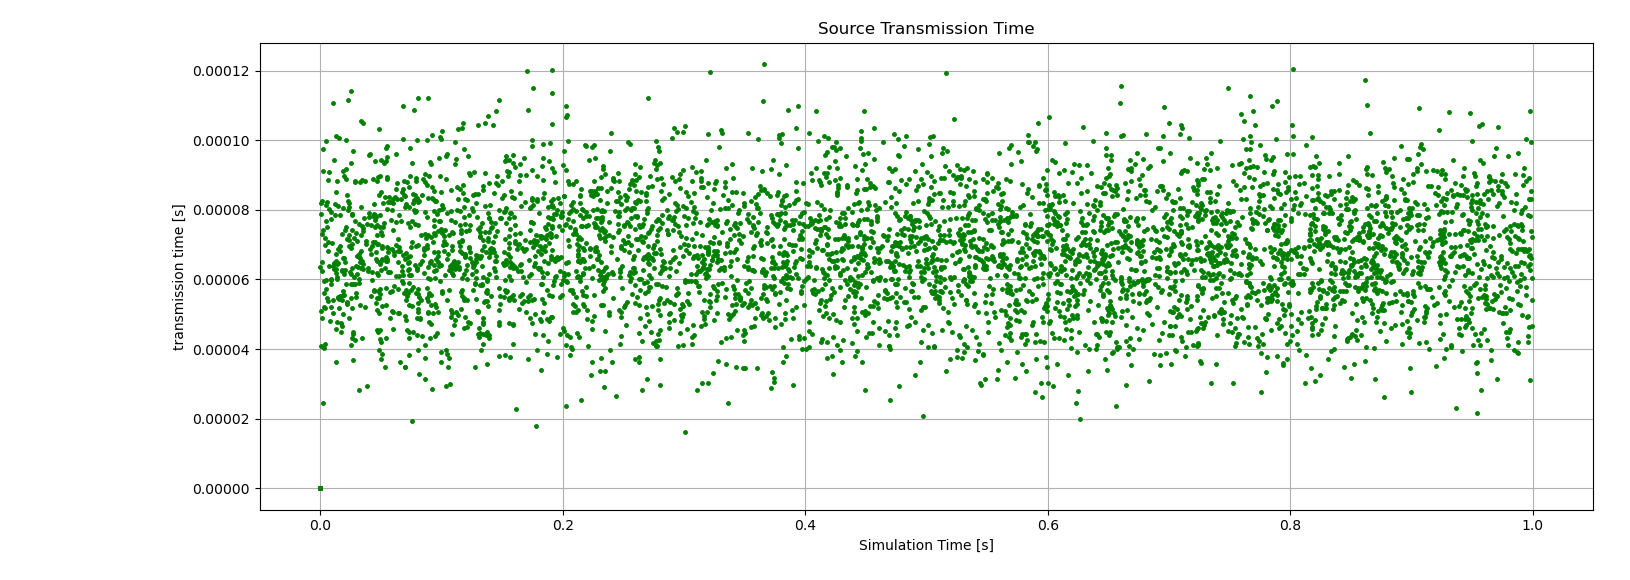
\includegraphics[width=0.8\linewidth]{screenshot011}
		\caption{Source Transmission Time}
		\label{fig:screenshot011}
	\end{figure}
	\begin{figure}[!h]
		\centering
		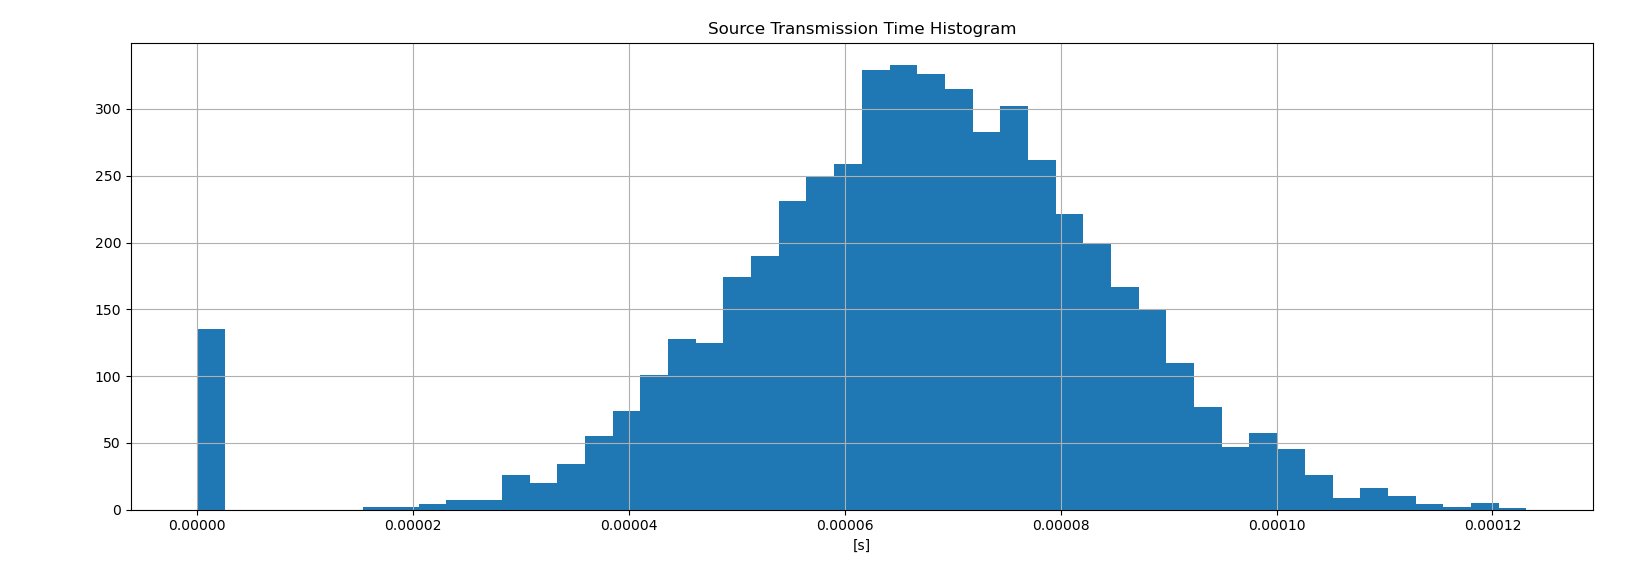
\includegraphics[width=0.8\linewidth]{screenshot012}
		\caption{Source Transmission Time Histogram}
		\label{fig:screenshot012}
	\end{figure}
	
	The simulation result of 67.89$\mu$s is higher than the expected value of 40$\mu$s. This is likely due to the randomness in the packet sizes generated by the truncated normal distribution, which may have resulted in a higher proportion of larger packets.
	The deviation in the result reflects the variability in transmission times caused by the random distribution of packet sizes. This is consistent with the fact that larger packets require more time to transmit, and smaller packets require less time.
	
	The difference between the simulation mean and the calculated mean transmission time is likely due to the random distribution of packet sizes, which may have resulted in larger packets on average in the simulation. In calculation I assumed an idealized mean packet size of 500 bytes, but the simulation data suggests that larger packets were generated more frequently or the distribution skewed towards larger sizes, resulting in a higher observed mean transmission time.
	
	\subsection{Measuring Data Rate}
	
	\begin{figure}[!h]
		\centering
		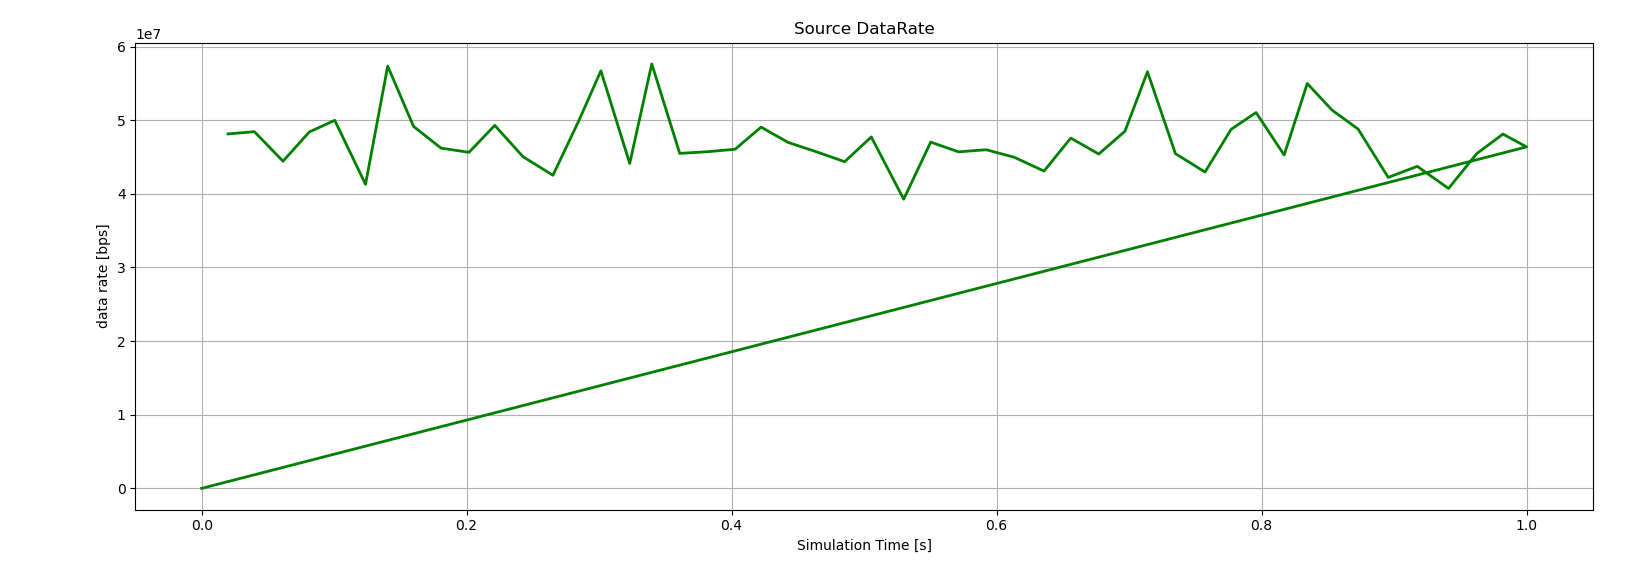
\includegraphics[width=0.8\linewidth]{screenshot013}
		\caption{}
		\label{fig:screenshot013}
	\end{figure}
	\begin{figure}[!h]
		\centering
		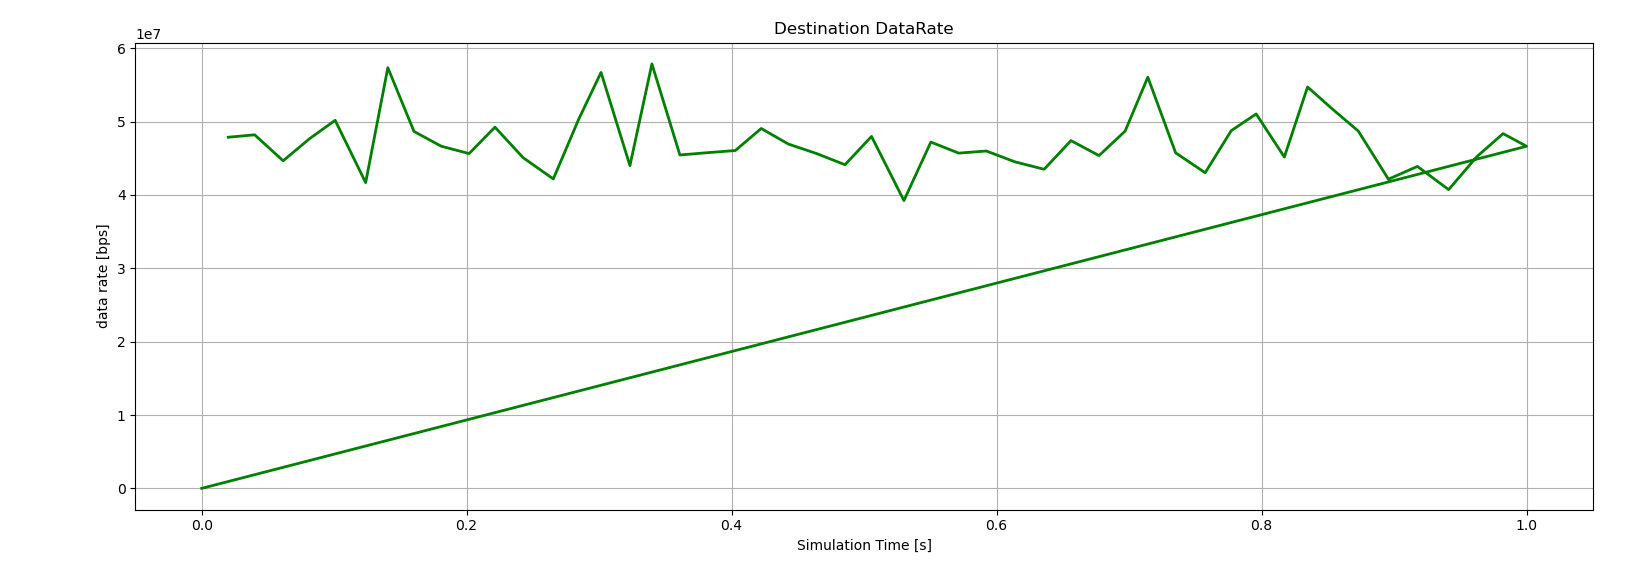
\includegraphics[width=0.8\linewidth]{screenshot014}
		\caption{}
		\label{fig:screenshot014}
	\end{figure}
	
	The source and destination data rates being nearly identical (47.237Mbps and 47.236Mbps, respectively) suggests that the network is functioning efficiently, with minimal packet loss or delay.
	
	The standard deviations of 4.13Mbps and 4.11Mbps show that there is some random fluctuation in the data rates due to the random nature of packet generation but that these fluctuations are not large enough to significantly affect the overall transmission efficiency.
	
	The source data rate is very close to the calculated expected throughput, which suggests that the network is performing well and not introducing significant inefficiencies.
	
	\pagebreak
	
	\section{Visualizing Data Link Activity}
	
	\subsection{Enabling Visualization of Data Link Activity}
	\large
	
	\Large
	a)
	\large
	\begin{figure}[!h]
		\centering
		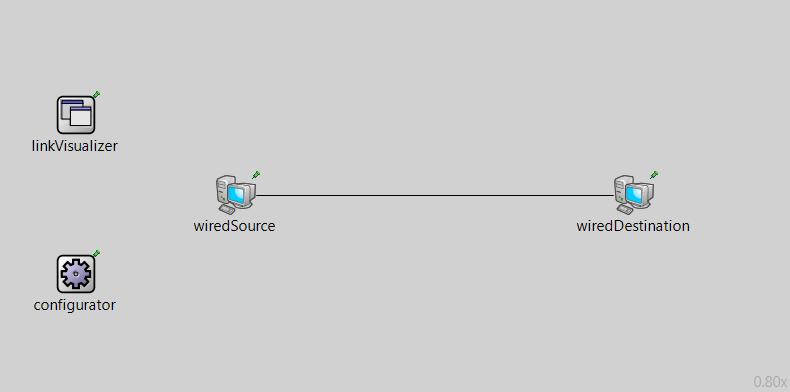
\includegraphics[width=0.7\linewidth]{screenshot015}
		\caption{Network Description}
		\label{fig:screenshot015}
	\end{figure}
	
	\Large
	b)
	\large
	\begin{figure}[h!]
		\centering
		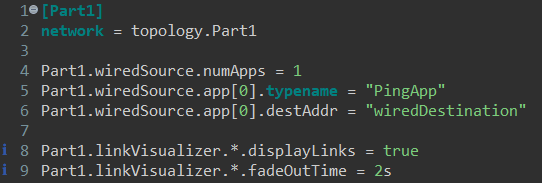
\includegraphics[width=0.7\linewidth]{screenshot016}
		\caption{Simulator Configurations}
		\label{fig:screenshot016}
	\end{figure}
	
	\Large
	c)
	\large
	\begin{center}
		\Large
		DataLink Activity
		
		\large
		\begin{figure}[!htb]
			\begin{minipage}{0.45\textwidth}
				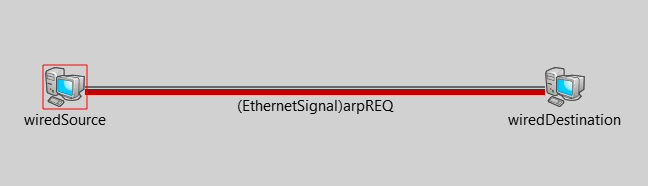
\includegraphics[width=\linewidth]{1}
			\end{minipage}\hfill
			\begin{minipage}{0.45\textwidth}
				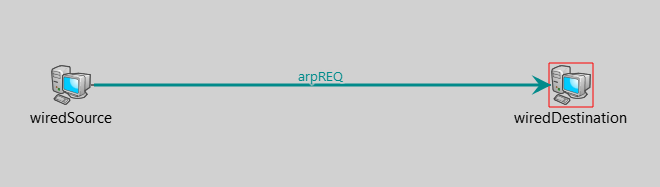
\includegraphics[width=\linewidth]{2}
			\end{minipage}\hfill
		\end{figure}
		\begin{figure}[!htb]
			\begin{minipage}{0.45\textwidth}
				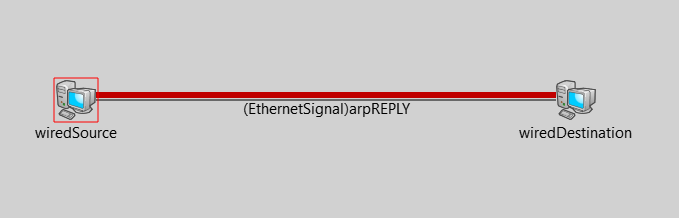
\includegraphics[width=\linewidth]{3}
			\end{minipage}\hfill
			\begin{minipage}{0.45\textwidth}
				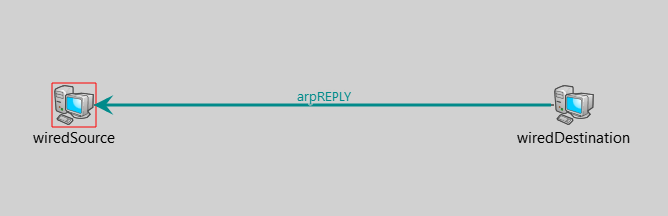
\includegraphics[width=\linewidth]{4}
			\end{minipage}\hfill
		\end{figure}
		
		ARP REQ and REPLY process
		\pagebreak
		
		\begin{figure}[!htb]
			\begin{minipage}{0.45\textwidth}
				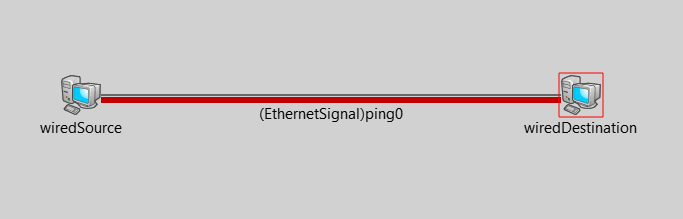
\includegraphics[width=\linewidth]{5}
			\end{minipage}\hfill
			\begin{minipage}{0.45\textwidth}
				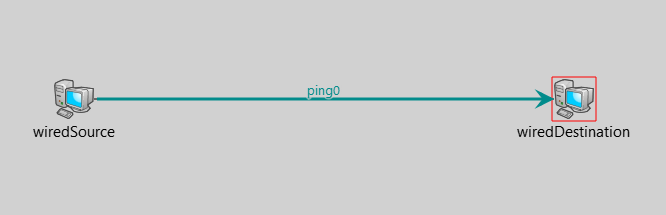
\includegraphics[width=\linewidth]{6}
			\end{minipage}\hfill
		\end{figure}
		\begin{figure}[!htb]
			\begin{minipage}{0.45\textwidth}
				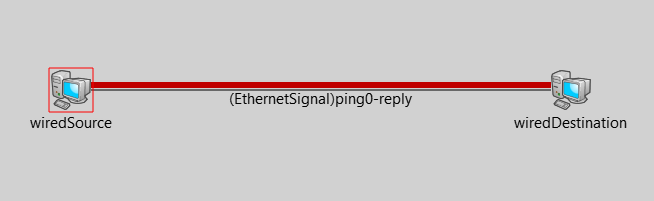
\includegraphics[width=\linewidth]{7}
			\end{minipage}\hfill
			\begin{minipage}{0.45\textwidth}
				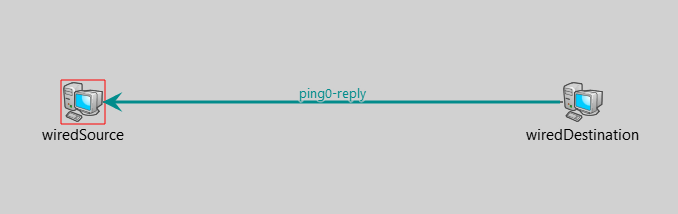
\includegraphics[width=\linewidth]{8}
			\end{minipage}\hfill
		\end{figure}
		
		ping transmission and reply
	\end{center}
	
	\subsection{Filtering Data Link Activity}
	\Large
	a)
	\large
	\begin{figure}[!h]
		\centering
		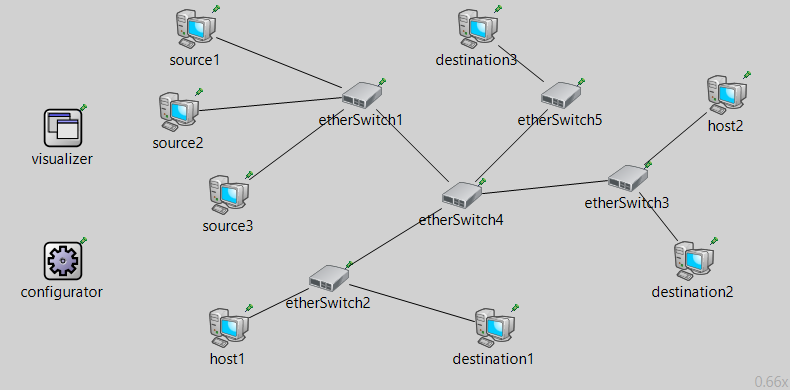
\includegraphics[width=0.7\linewidth]{screenshot017}
		\caption{Network Description}
		\label{fig:screenshot017}
	\end{figure}
	
	\begin{figure}[h!]
		\centering
		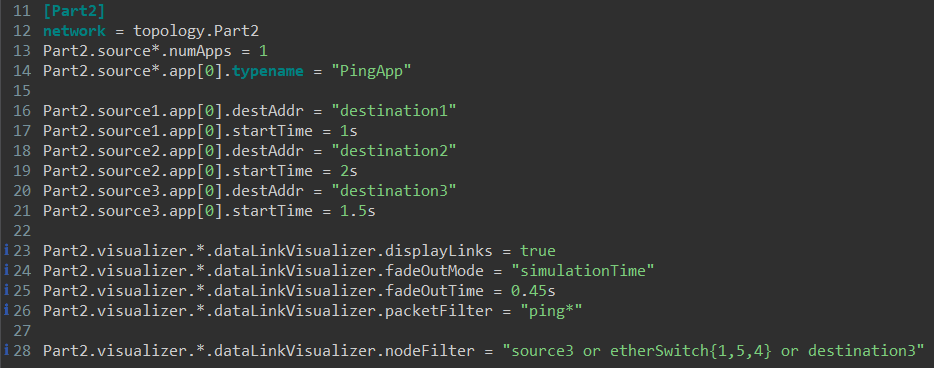
\includegraphics[width=0.7\linewidth]{screenshot018}
		\caption{Simulator Configurations}
		\label{fig:screenshot018}
	\end{figure}
	
	\pagebreak
	
	\Large
	b)
	\large
	
	As you can see below, \textit{source1} first requests to establish connection with \textit{destination1}. Then \textit{destination1} replies to that request and the connection is established. After that \textit{source1} starts to send \textit{ping0} message and when the packet is received in whole by a host, a dark cyan arrow is added by DataLinkVisualizer between the two hosts, indicating data link activity. You can see the same process for \textit{source2} and \textit{destination2}.
		\begin{center}
		\Large
		DataLink Activity with Filtering
		
		\large
		\begin{figure}[!htb]
			\begin{minipage}{0.45\textwidth}
				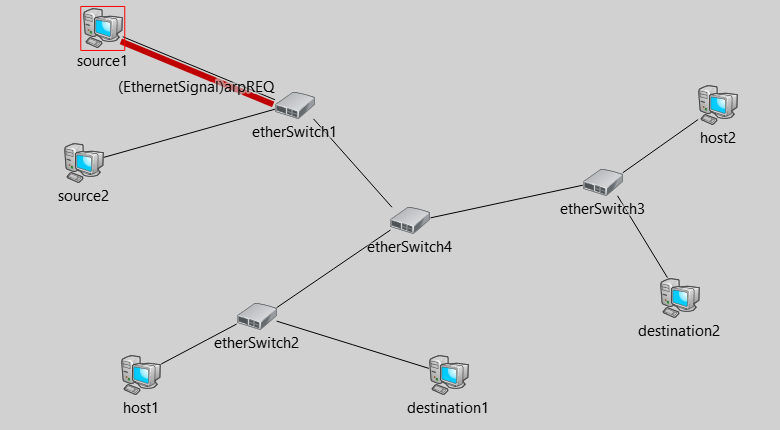
\includegraphics[width=\linewidth]{9}
			\end{minipage}\hfill
			\begin{minipage}{0.45\textwidth}
				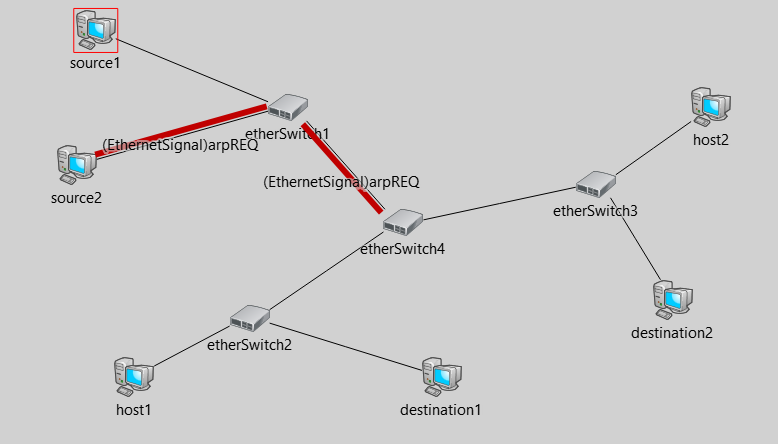
\includegraphics[width=\linewidth]{10}
			\end{minipage}\hfill
		\end{figure}
		\begin{figure}[!htb]
			\begin{minipage}{0.45\textwidth}
				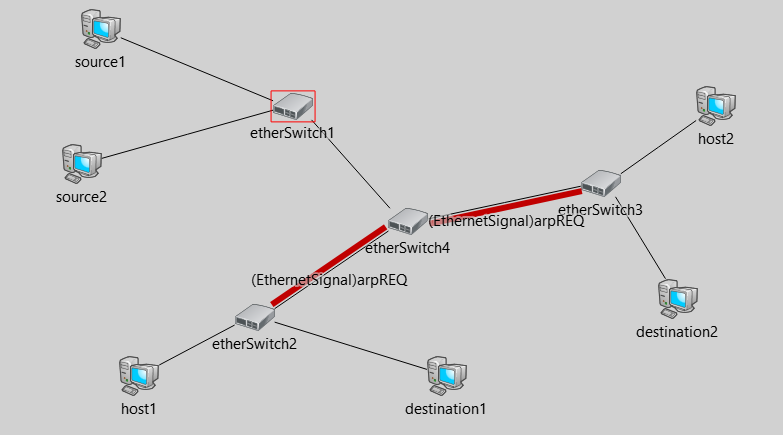
\includegraphics[width=\linewidth]{11}
			\end{minipage}\hfill
			\begin{minipage}{0.45\textwidth}
				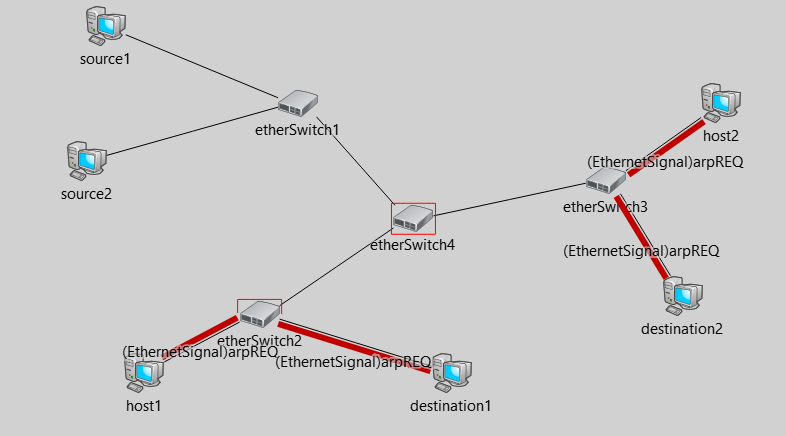
\includegraphics[width=\linewidth]{12}
			\end{minipage}\hfill
		\end{figure}
		\begin{figure}[!htb]
			\begin{minipage}{0.45\textwidth}
				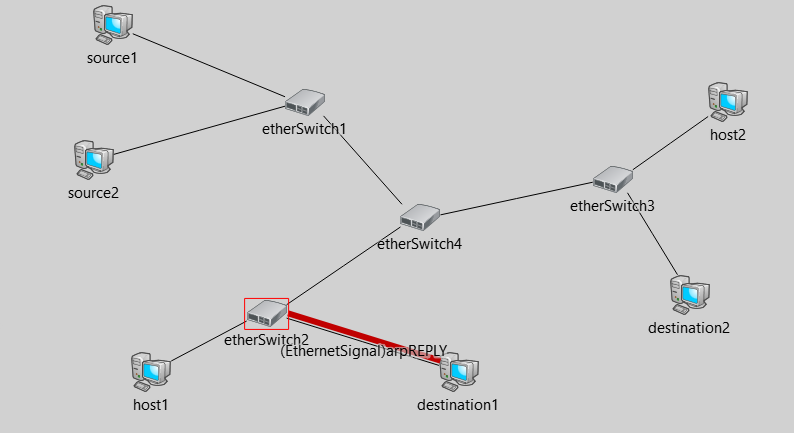
\includegraphics[width=\linewidth]{13}
			\end{minipage}\hfill
			\begin{minipage}{0.45\textwidth}
				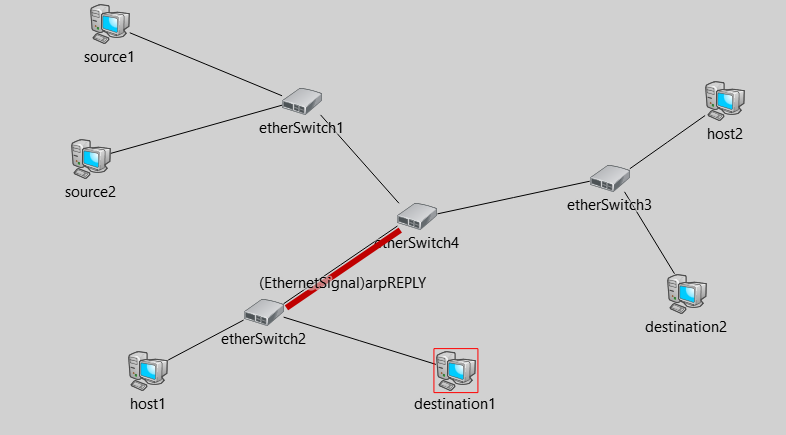
\includegraphics[width=\linewidth]{14}
			\end{minipage}\hfill
		\end{figure}
		\begin{figure}[!htb]
			\begin{minipage}{0.45\textwidth}
				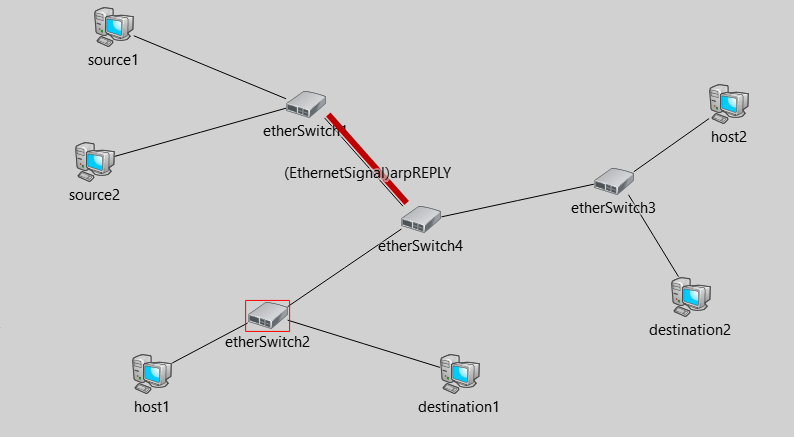
\includegraphics[width=\linewidth]{15}
			\end{minipage}\hfill
			\begin{minipage}{0.45\textwidth}
				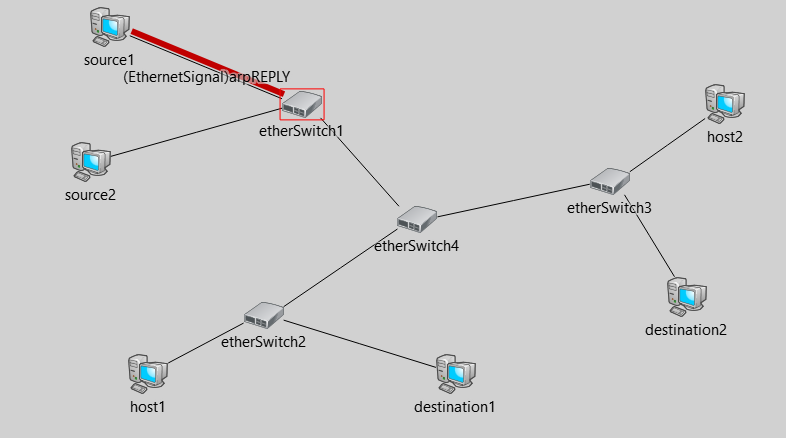
\includegraphics[width=\linewidth]{16}
			\end{minipage}\hfill
		\end{figure}
		
		\pagebreak
		
		\begin{figure}[!htb]
			\begin{minipage}{0.45\textwidth}
				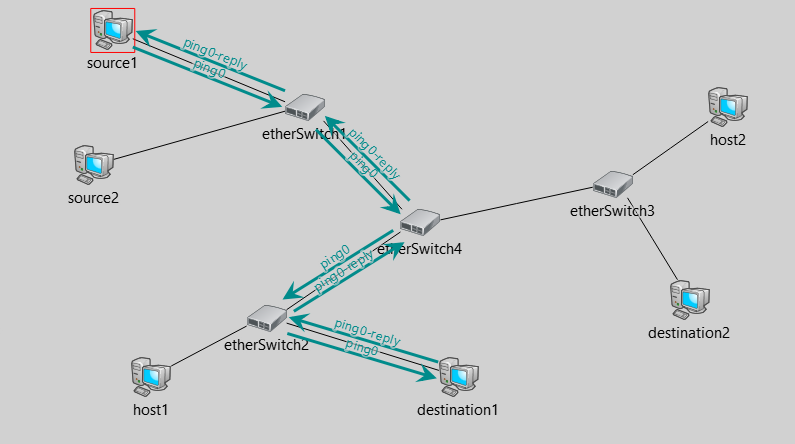
\includegraphics[width=\linewidth]{17}
			\end{minipage}\hfill
			\begin{minipage}{0.45\textwidth}
				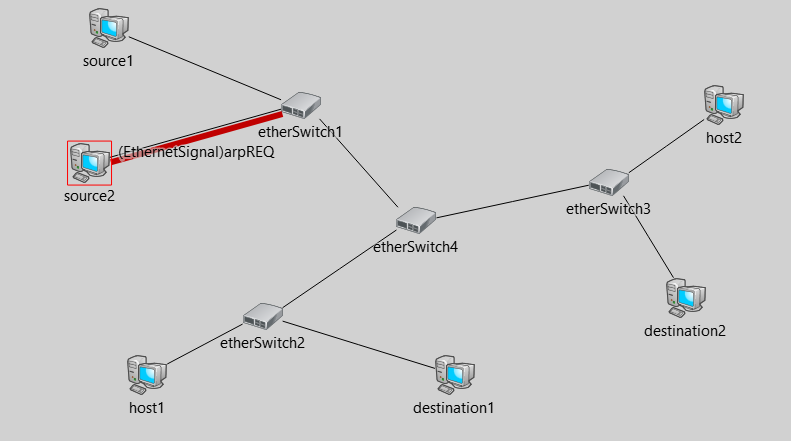
\includegraphics[width=\linewidth]{18}
			\end{minipage}\hfill
		\end{figure}
		\begin{figure}[!htb]
			\begin{minipage}{0.45\textwidth}
				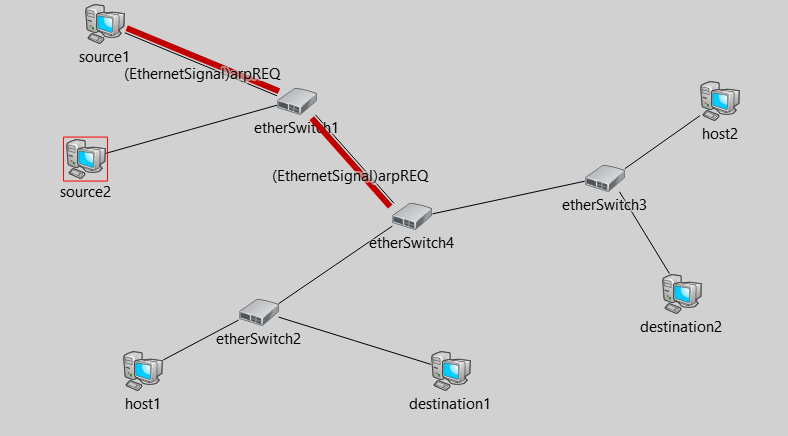
\includegraphics[width=\linewidth]{19}
			\end{minipage}\hfill
			\begin{minipage}{0.45\textwidth}
				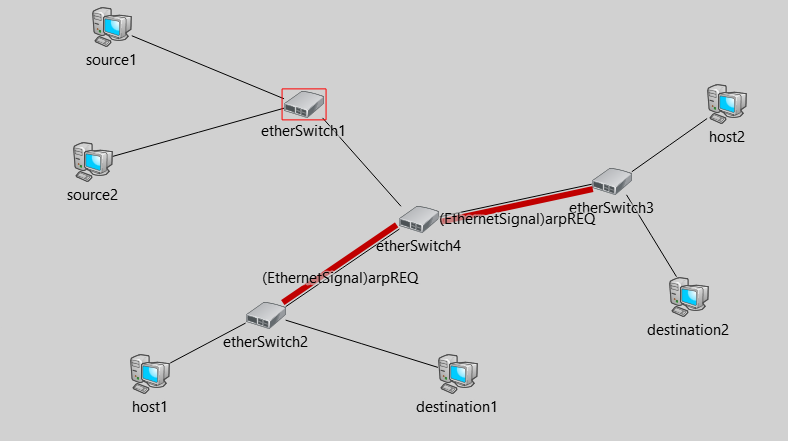
\includegraphics[width=\linewidth]{20}
			\end{minipage}\hfill
		\end{figure}
		\begin{figure}[!htb]
			\begin{minipage}{0.45\textwidth}
				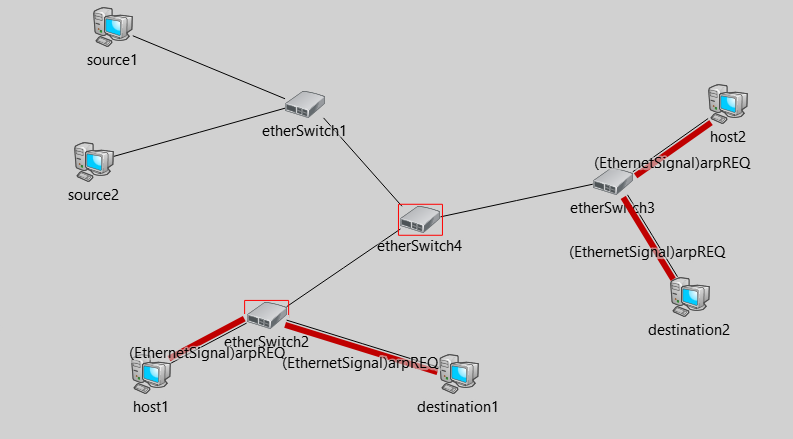
\includegraphics[width=\linewidth]{21}
			\end{minipage}\hfill
			\begin{minipage}{0.45\textwidth}
				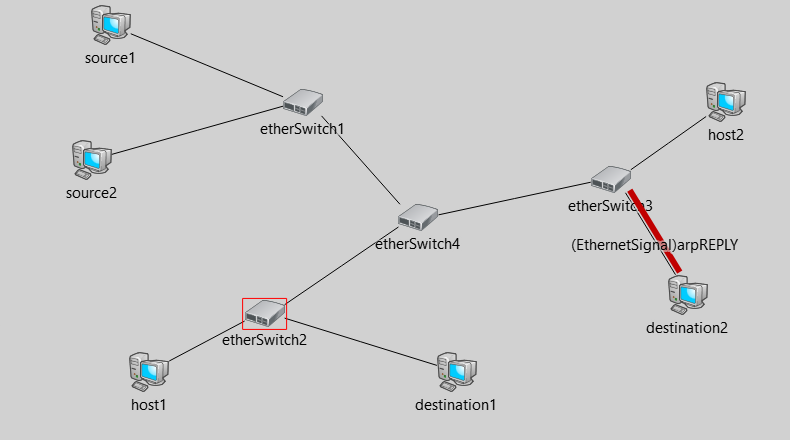
\includegraphics[width=\linewidth]{22}
			\end{minipage}\hfill
		\end{figure}
		\begin{figure}[!htb]
			\begin{minipage}{0.45\textwidth}
				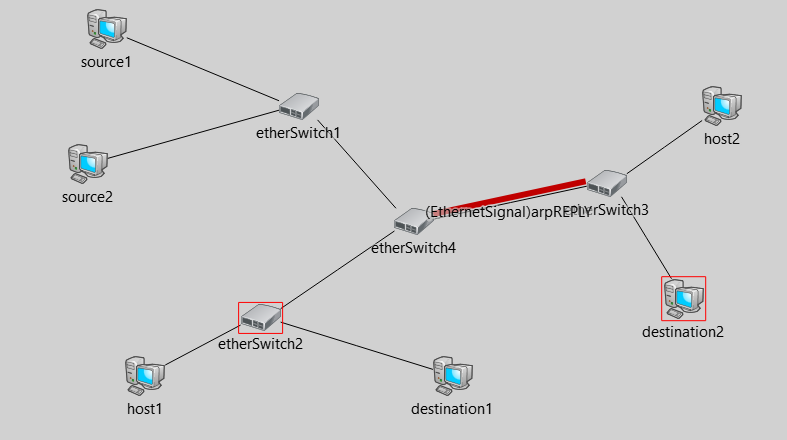
\includegraphics[width=\linewidth]{23}
			\end{minipage}\hfill
			\begin{minipage}{0.45\textwidth}
				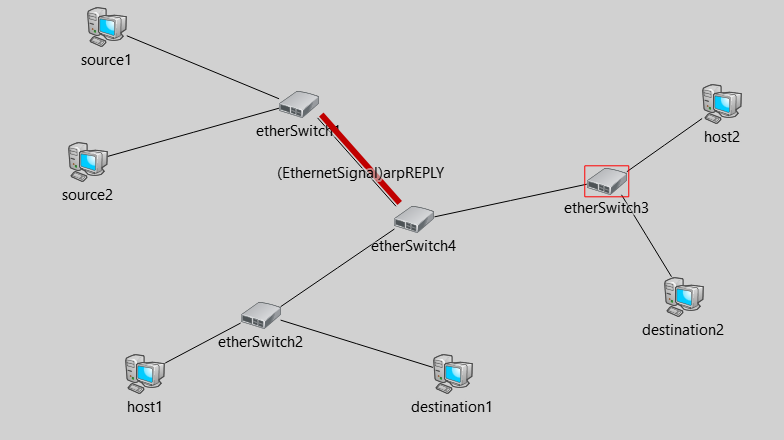
\includegraphics[width=\linewidth]{24}
			\end{minipage}\hfill
		\end{figure}
		\begin{figure}[!htb]
			\begin{minipage}{0.45\textwidth}
				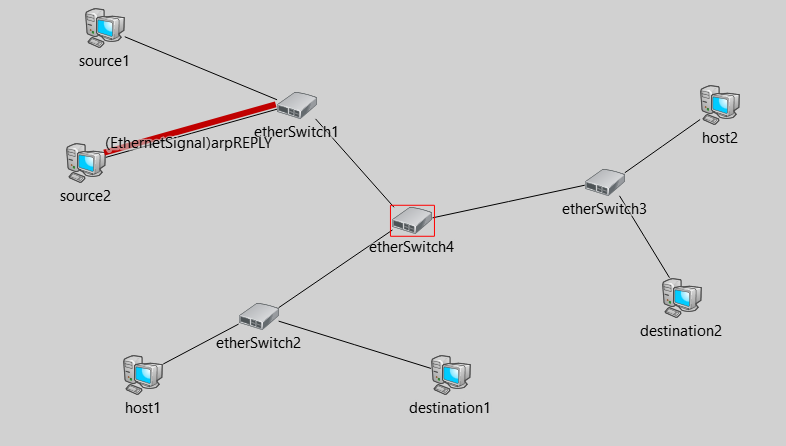
\includegraphics[width=\linewidth]{25}
			\end{minipage}\hfill
			\begin{minipage}{0.45\textwidth}
				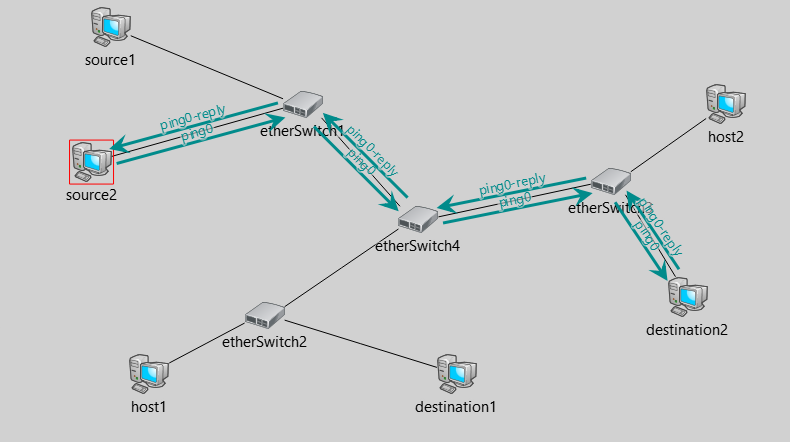
\includegraphics[width=\linewidth]{26}
			\end{minipage}\hfill
		\end{figure}
	\end{center}
	
	\pagebreak
	
	\Large
	c)
	\large
	\begin{center}
		\begin{figure}[!htb]
			\begin{minipage}{0.45\textwidth}
				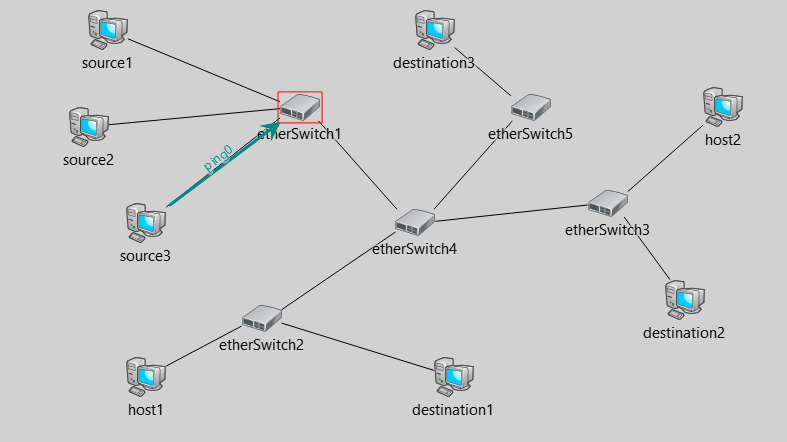
\includegraphics[width=\linewidth]{27}
			\end{minipage}\hfill
			\begin{minipage}{0.45\textwidth}
				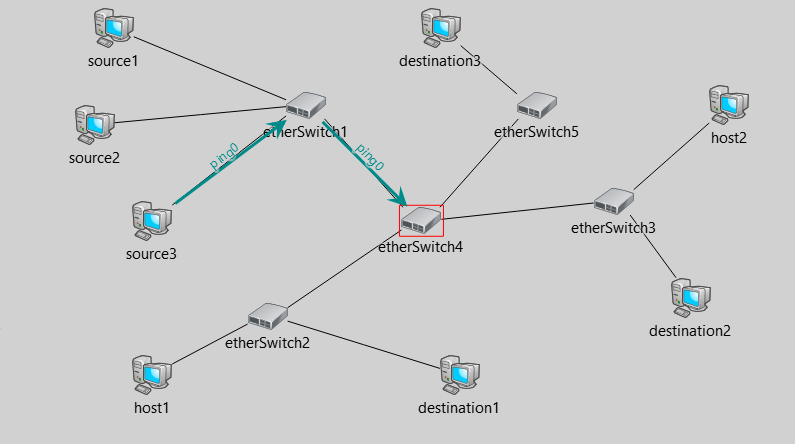
\includegraphics[width=\linewidth]{28}
			\end{minipage}\hfill
		\end{figure}
		\begin{figure}[!htb]
			\begin{minipage}{0.45\textwidth}
				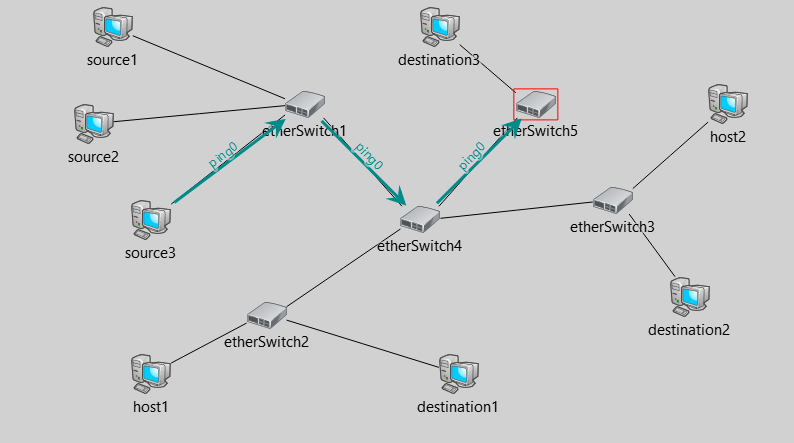
\includegraphics[width=\linewidth]{29}
			\end{minipage}\hfill
			\begin{minipage}{0.45\textwidth}
				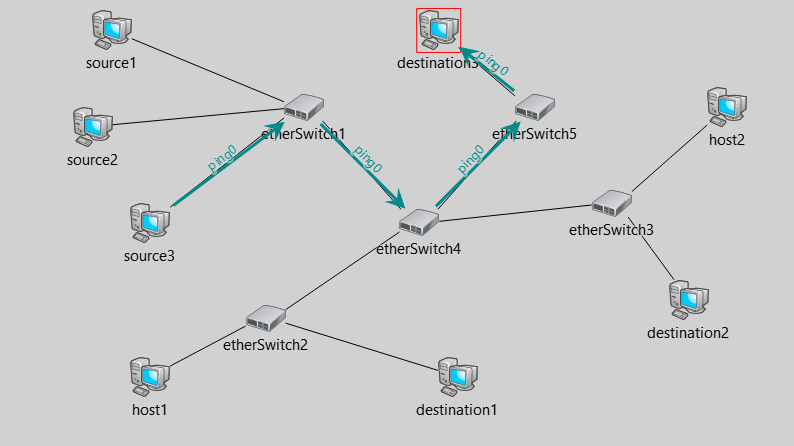
\includegraphics[width=\linewidth]{30}
			\end{minipage}\hfill
		\end{figure}
		\begin{figure}[!htb]
			\begin{minipage}{0.45\textwidth}
				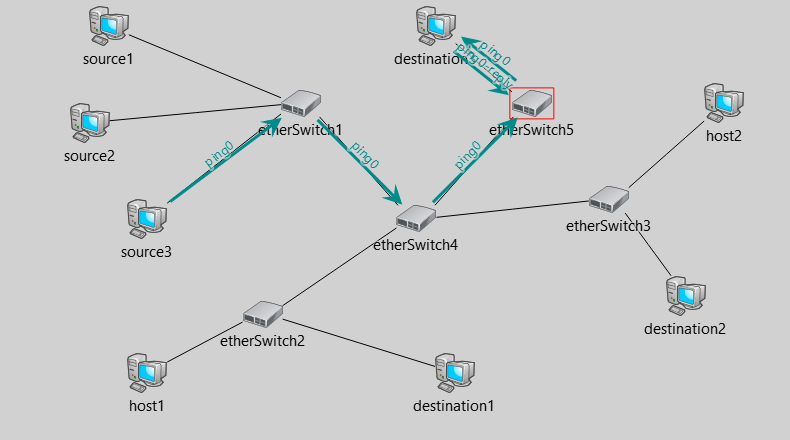
\includegraphics[width=\linewidth]{31}
			\end{minipage}\hfill
			\begin{minipage}{0.45\textwidth}
				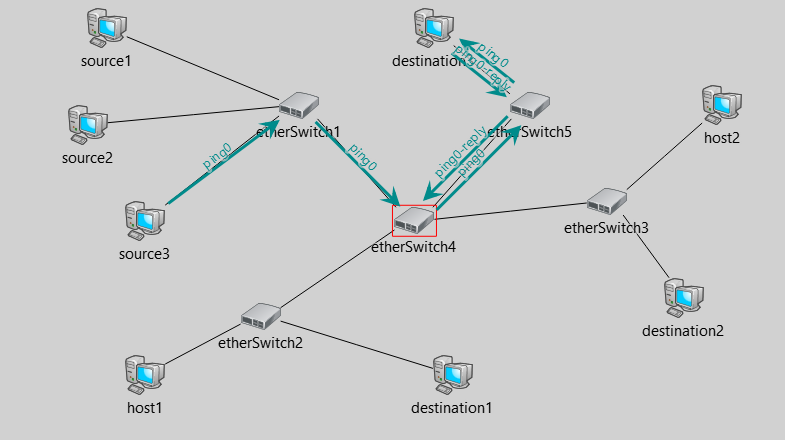
\includegraphics[width=\linewidth]{32}
			\end{minipage}\hfill
		\end{figure}
		\begin{figure}[!htb]
			\begin{minipage}{0.45\textwidth}
				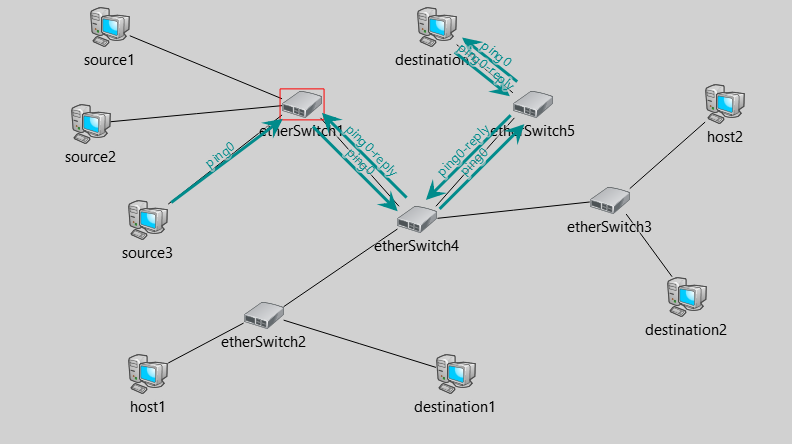
\includegraphics[width=\linewidth]{33}
			\end{minipage}\hfill
			\begin{minipage}{0.45\textwidth}
				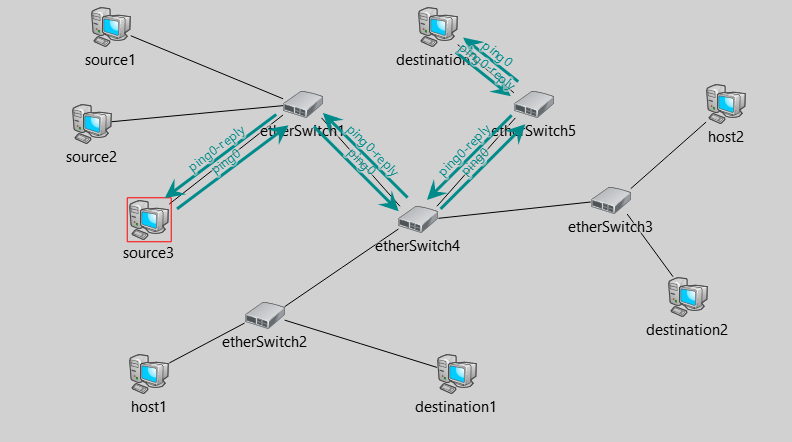
\includegraphics[width=\linewidth]{34}
			\end{minipage}\hfill
		\end{figure}
		\begin{figure}[!htb]
			\begin{minipage}{0.45\textwidth}
				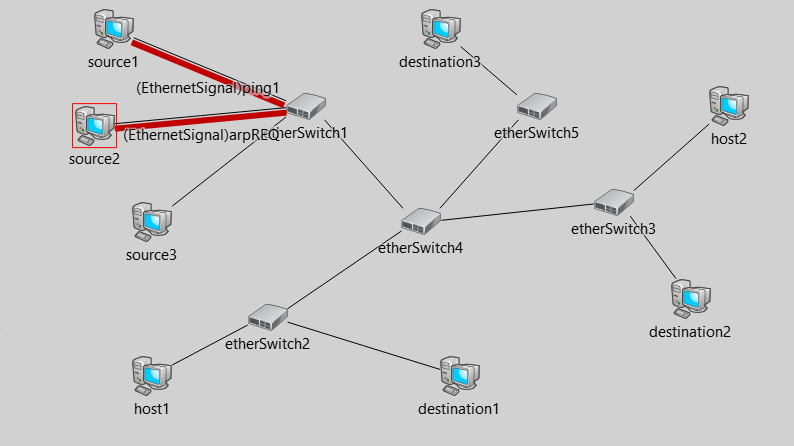
\includegraphics[width=\linewidth]{35}
			\end{minipage}\hfill
			\begin{minipage}{0.45\textwidth}
				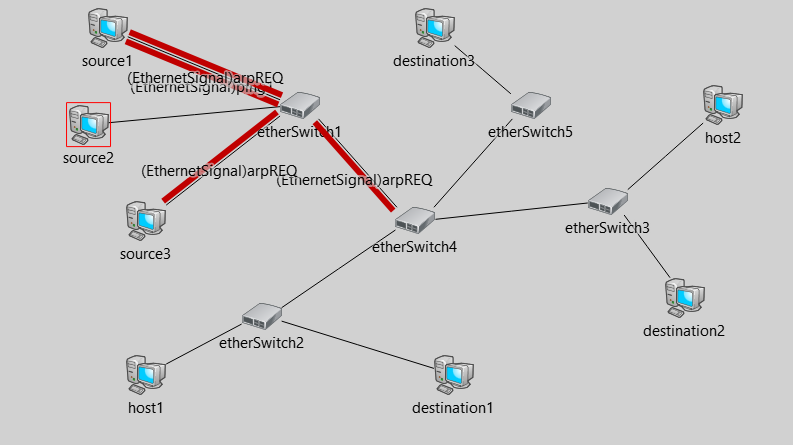
\includegraphics[width=\linewidth]{36}
			\end{minipage}\hfill
		\end{figure}
		
		\pagebreak
		
		\begin{figure}[!htb]
			\begin{minipage}{0.45\textwidth}
				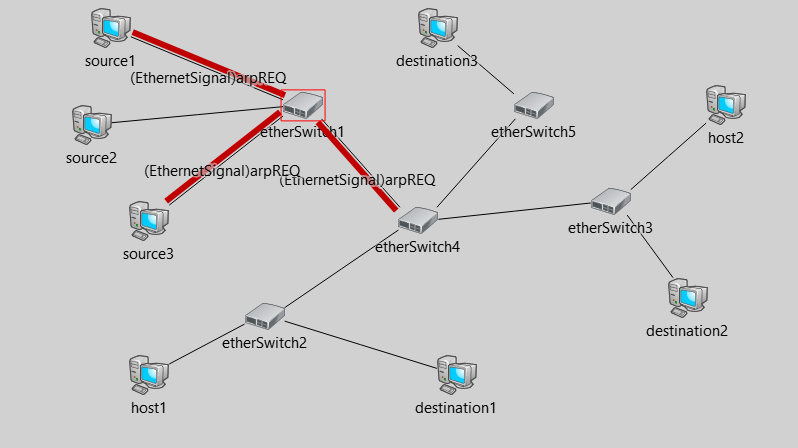
\includegraphics[width=\linewidth]{37}
			\end{minipage}\hfill
			\begin{minipage}{0.45\textwidth}
				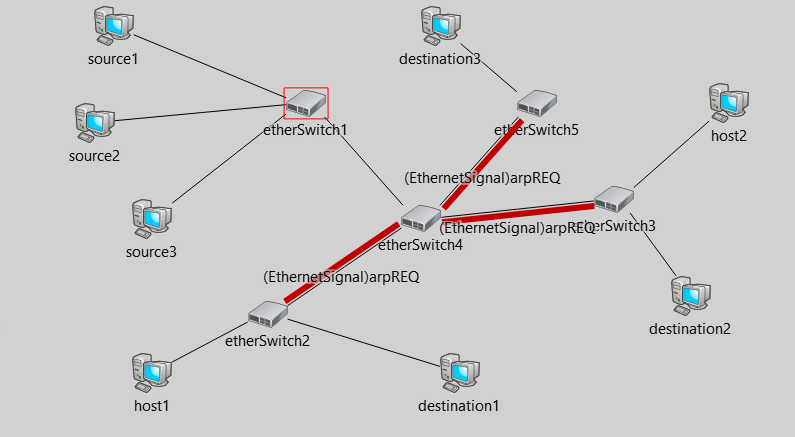
\includegraphics[width=\linewidth]{38}
			\end{minipage}\hfill
		\end{figure}
		\begin{figure}[!htb]
			\begin{minipage}{0.45\textwidth}
				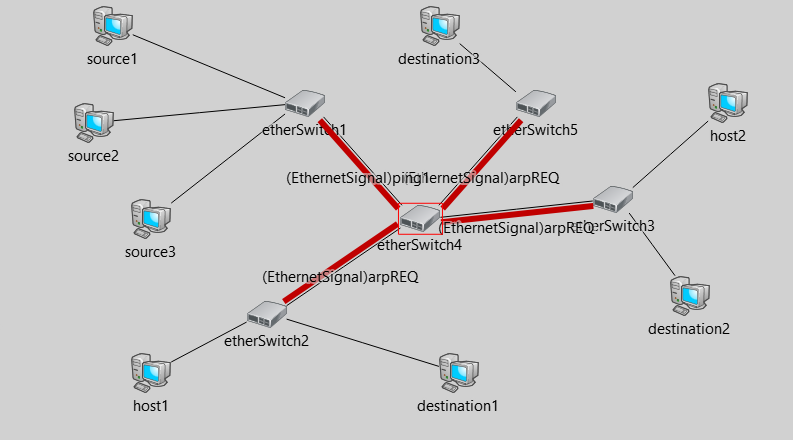
\includegraphics[width=\linewidth]{39}
			\end{minipage}\hfill
			\begin{minipage}{0.45\textwidth}
				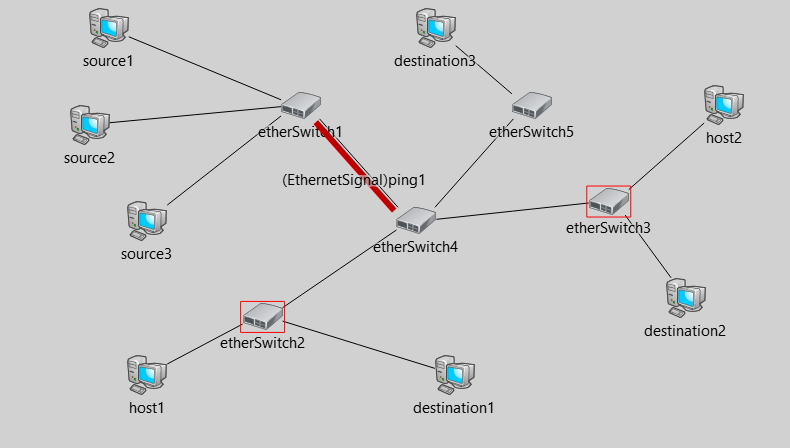
\includegraphics[width=\linewidth]{40}
			\end{minipage}\hfill
		\end{figure}
		\begin{figure}[!htb]
			\begin{minipage}{0.45\textwidth}
				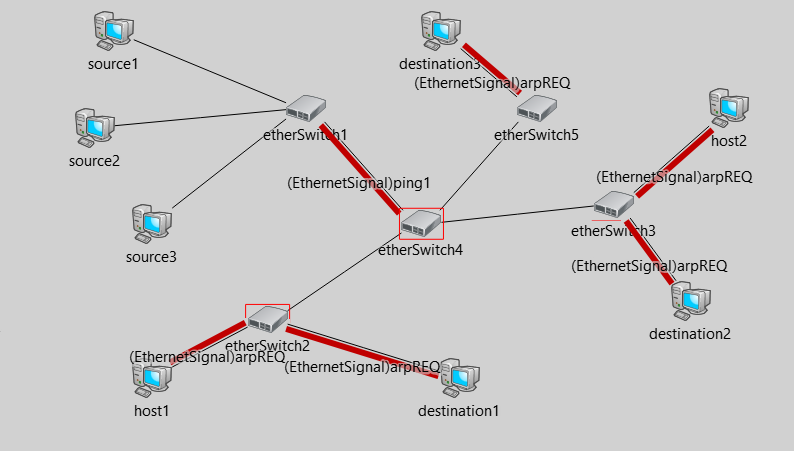
\includegraphics[width=\linewidth]{41}
			\end{minipage}\hfill
			\begin{minipage}{0.45\textwidth}
				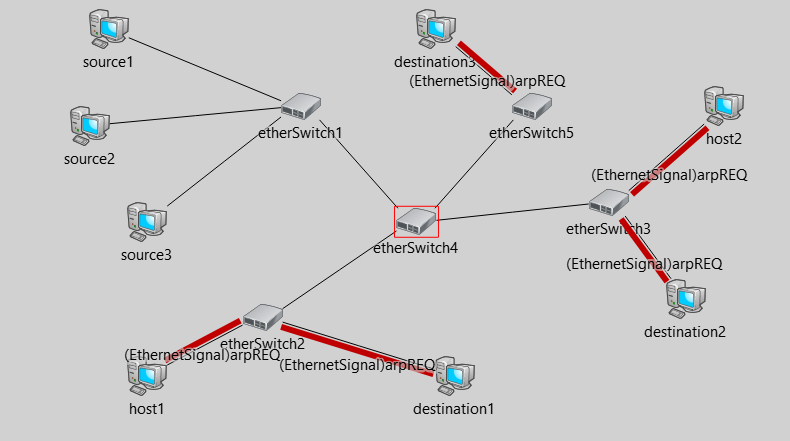
\includegraphics[width=\linewidth]{42}
			\end{minipage}\hfill
		\end{figure}
		\begin{figure}[!htb]
			\begin{minipage}{0.45\textwidth}
				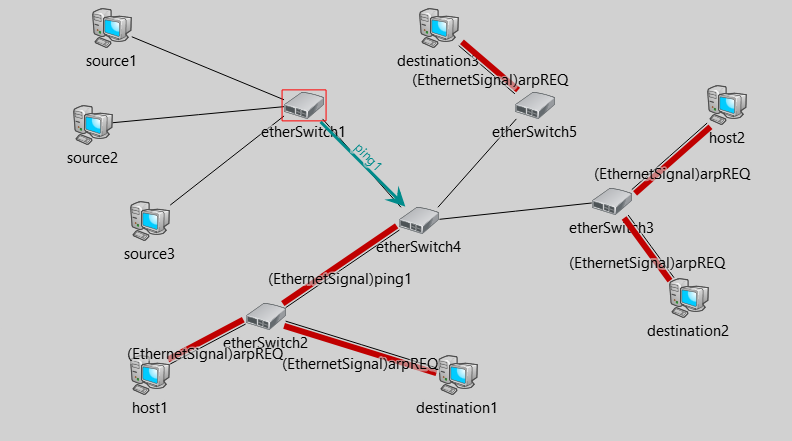
\includegraphics[width=\linewidth]{43}
			\end{minipage}\hfill
			\begin{minipage}{0.45\textwidth}
				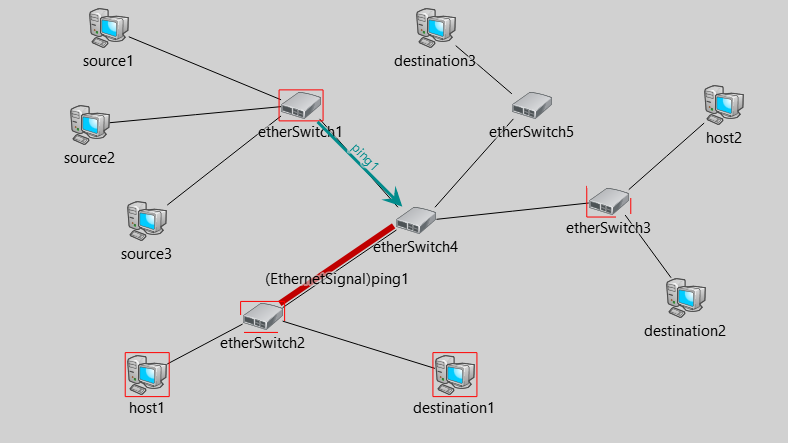
\includegraphics[width=\linewidth]{44}
			\end{minipage}\hfill
		\end{figure}
		\begin{figure}[!htb]
			\begin{minipage}{0.45\textwidth}
				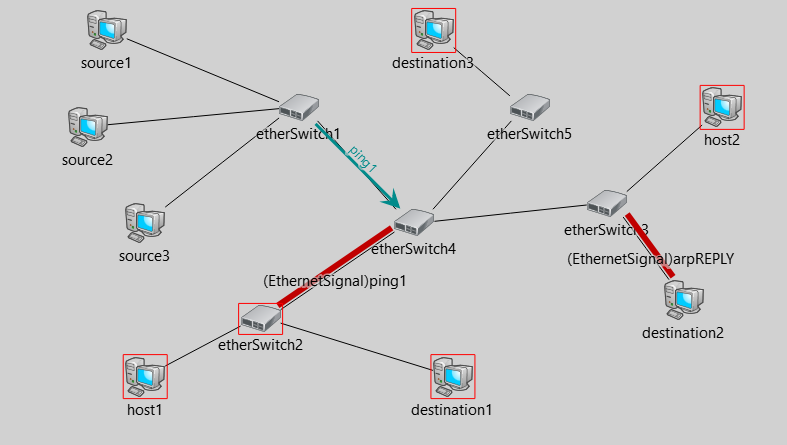
\includegraphics[width=\linewidth]{45}
			\end{minipage}\hfill
			\begin{minipage}{0.45\textwidth}
				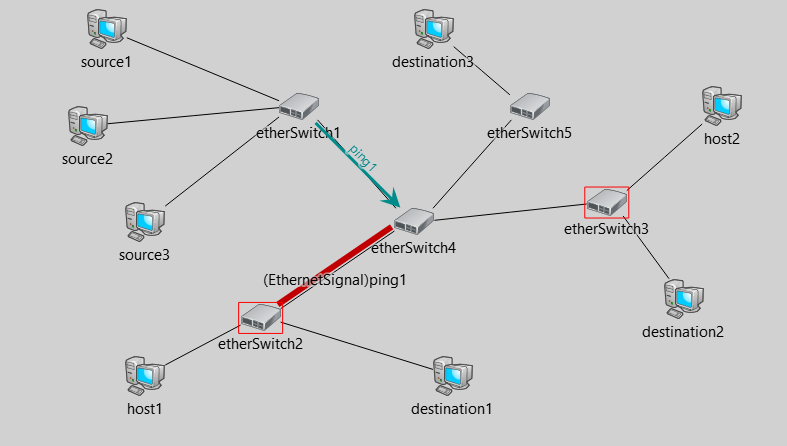
\includegraphics[width=\linewidth]{46}
			\end{minipage}\hfill
		\end{figure}
		
		\pagebreak
		
		\begin{figure}[!htb]
			\begin{minipage}{0.45\textwidth}
				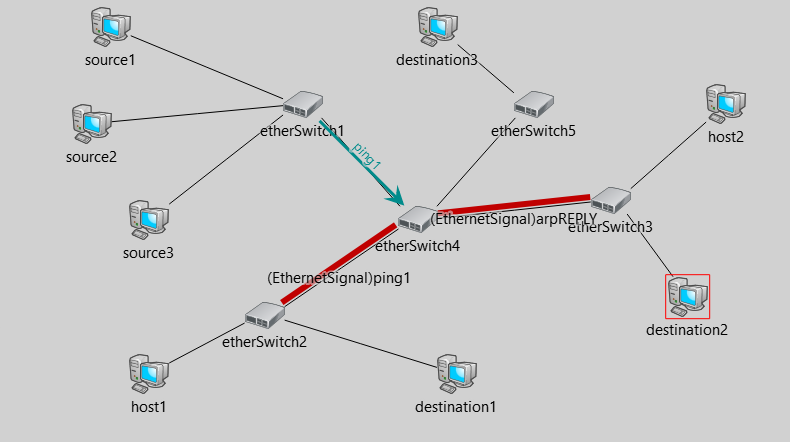
\includegraphics[width=\linewidth]{47}
			\end{minipage}\hfill
			\begin{minipage}{0.45\textwidth}
				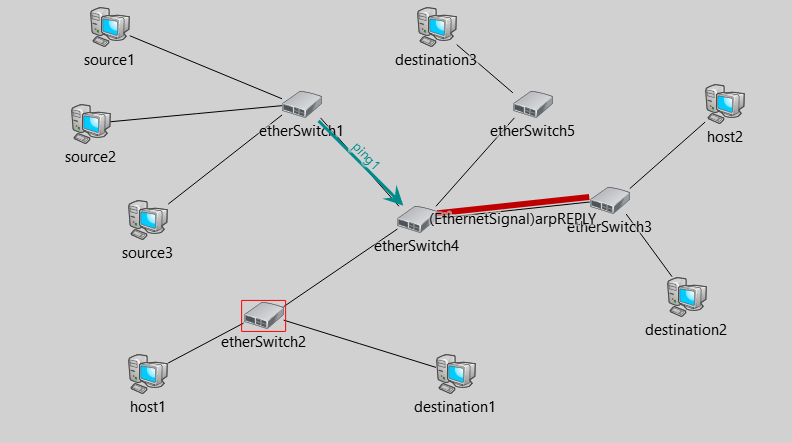
\includegraphics[width=\linewidth]{48}
			\end{minipage}\hfill
		\end{figure}
		\begin{figure}[!htb]
			\begin{minipage}{0.45\textwidth}
				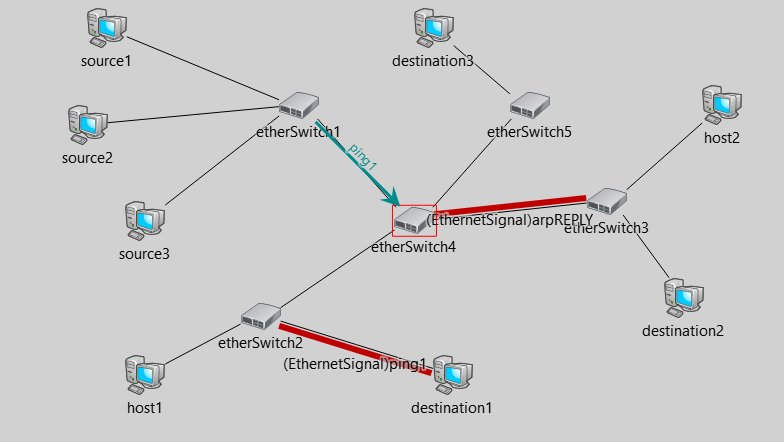
\includegraphics[width=\linewidth]{49}
			\end{minipage}\hfill
			\begin{minipage}{0.45\textwidth}
				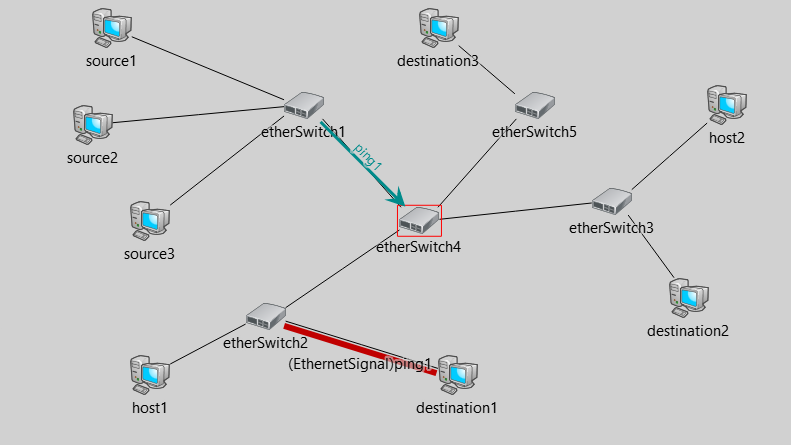
\includegraphics[width=\linewidth]{50}
			\end{minipage}\hfill
		\end{figure}
		\begin{figure}[!htb]
			\begin{minipage}{0.45\textwidth}
				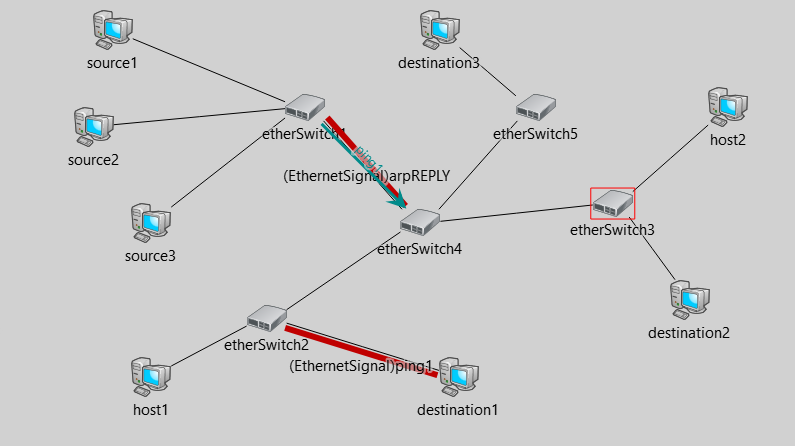
\includegraphics[width=\linewidth]{51}
			\end{minipage}\hfill
			\begin{minipage}{0.45\textwidth}
				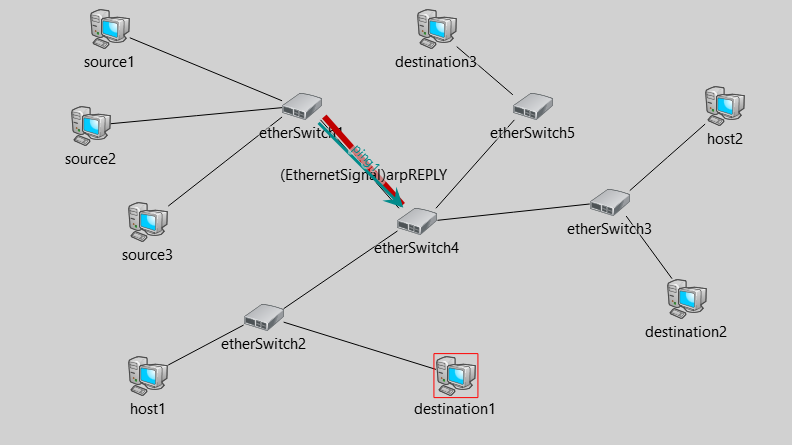
\includegraphics[width=\linewidth]{52}
			\end{minipage}\hfill
		\end{figure}
		\begin{figure}[!htb]
			\begin{minipage}{0.45\textwidth}
				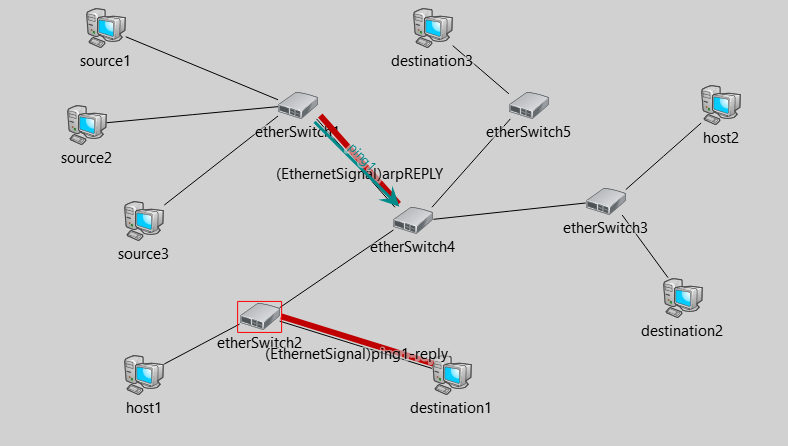
\includegraphics[width=\linewidth]{53}
			\end{minipage}\hfill
			\begin{minipage}{0.45\textwidth}
				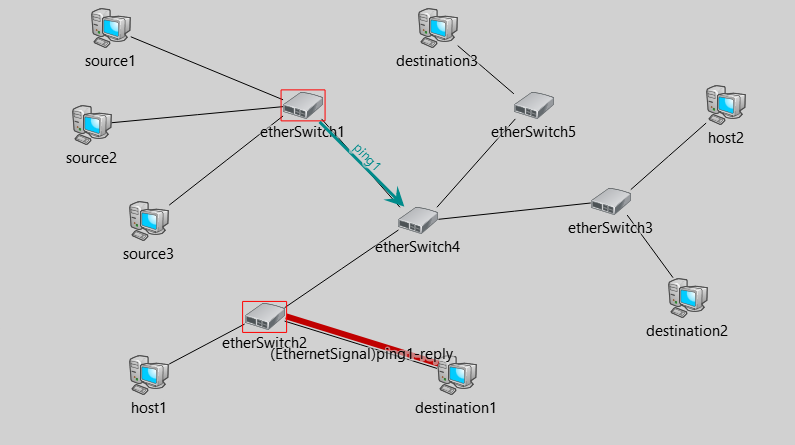
\includegraphics[width=\linewidth]{54}
			\end{minipage}\hfill
		\end{figure}
		\begin{figure}[!htb]
			\begin{minipage}{0.45\textwidth}
				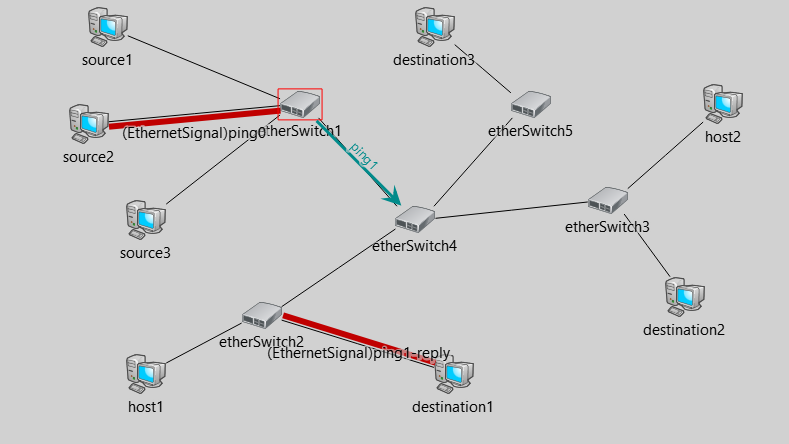
\includegraphics[width=\linewidth]{55}
			\end{minipage}\hfill
			\begin{minipage}{0.45\textwidth}
				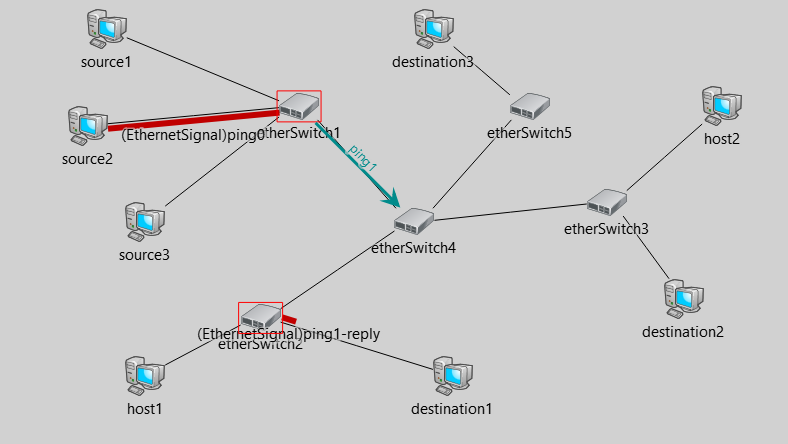
\includegraphics[width=\linewidth]{56}
			\end{minipage}\hfill
		\end{figure}
		
		\pagebreak
		
		\begin{figure}[!htb]
			\begin{minipage}{0.45\textwidth}
				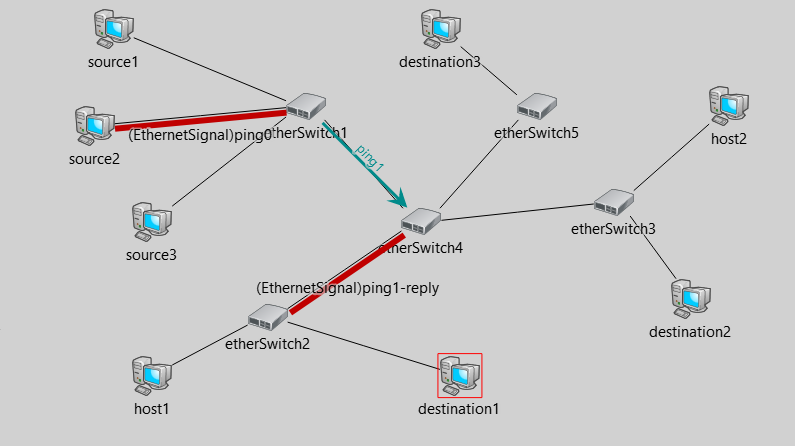
\includegraphics[width=\linewidth]{57}
			\end{minipage}\hfill
			\begin{minipage}{0.45\textwidth}
				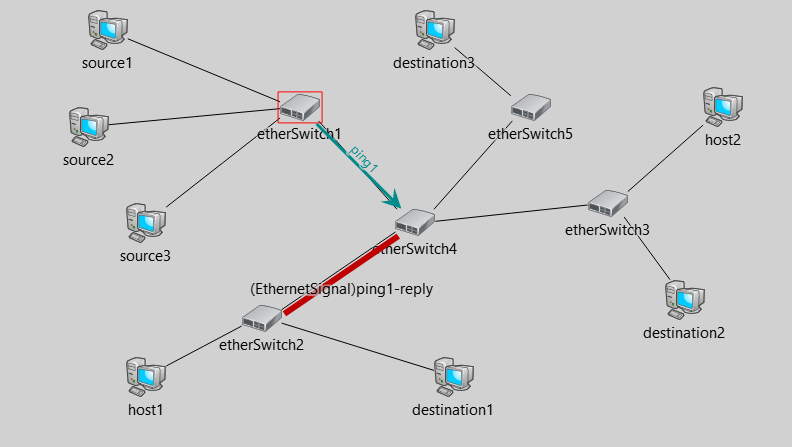
\includegraphics[width=\linewidth]{58}
			\end{minipage}\hfill
		\end{figure}
		\begin{figure}[!htb]
			\begin{minipage}{0.45\textwidth}
				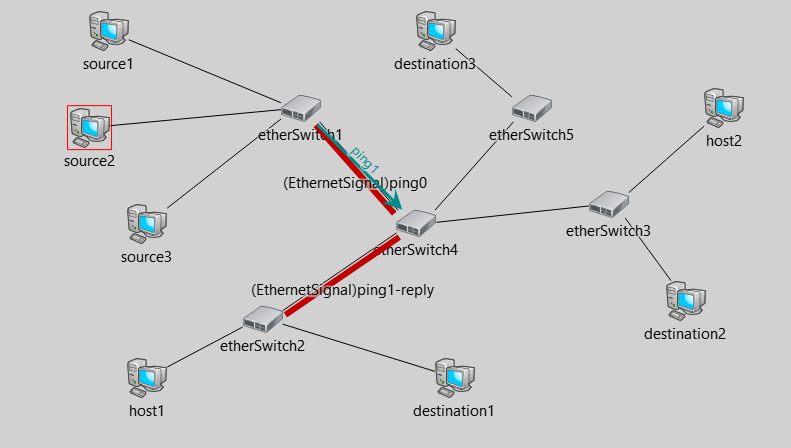
\includegraphics[width=\linewidth]{59}
			\end{minipage}\hfill
			\begin{minipage}{0.45\textwidth}
				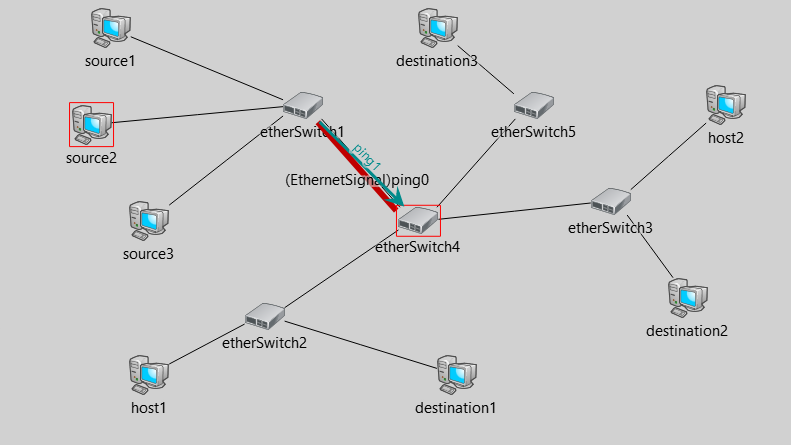
\includegraphics[width=\linewidth]{60}
			\end{minipage}\hfill
		\end{figure}
		\begin{figure}[!htb]
			\begin{minipage}{0.45\textwidth}
				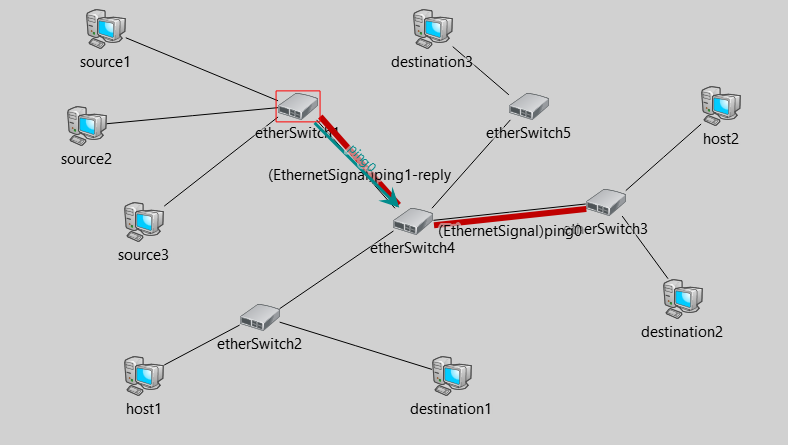
\includegraphics[width=\linewidth]{61}
			\end{minipage}\hfill
			\begin{minipage}{0.45\textwidth}
				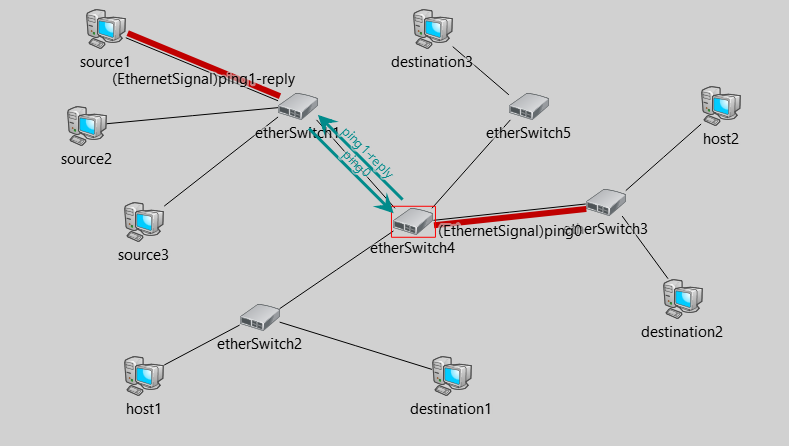
\includegraphics[width=\linewidth]{62}
			\end{minipage}\hfill
		\end{figure}
		\begin{figure}[!htb]
			\begin{minipage}{0.45\textwidth}
				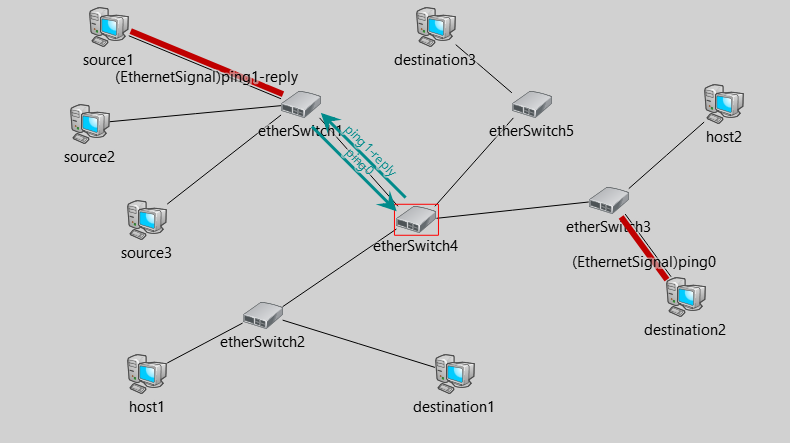
\includegraphics[width=\linewidth]{63}
			\end{minipage}\hfill
			\begin{minipage}{0.45\textwidth}
				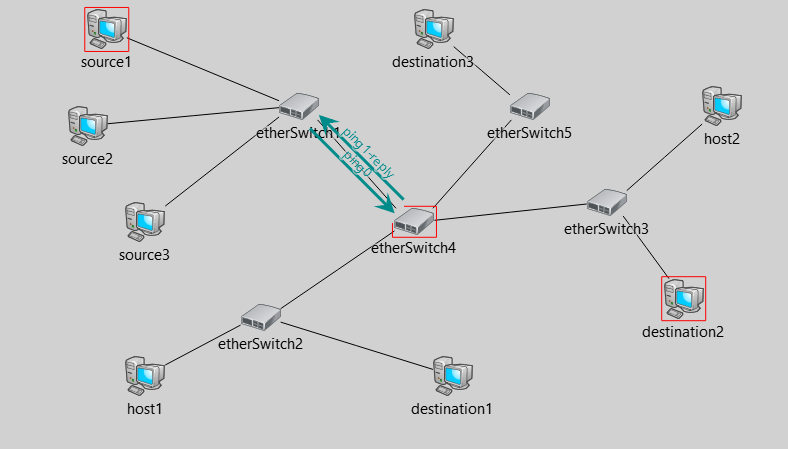
\includegraphics[width=\linewidth]{64}
			\end{minipage}\hfill
		\end{figure}
		\begin{figure}[!htb]
			\begin{minipage}{0.45\textwidth}
				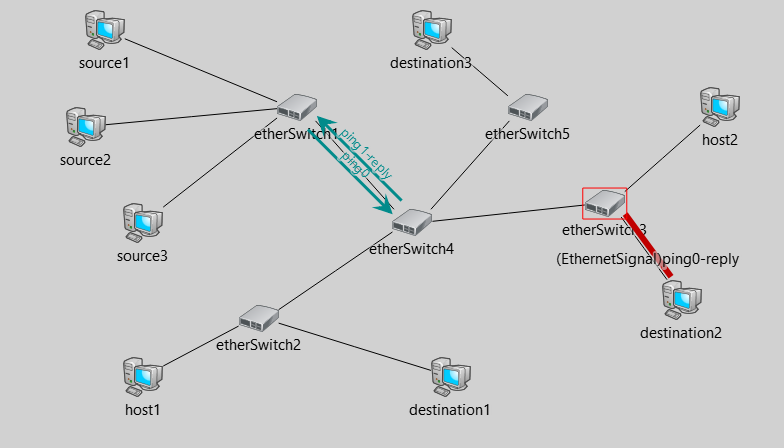
\includegraphics[width=\linewidth]{65}
			\end{minipage}\hfill
			\begin{minipage}{0.45\textwidth}
				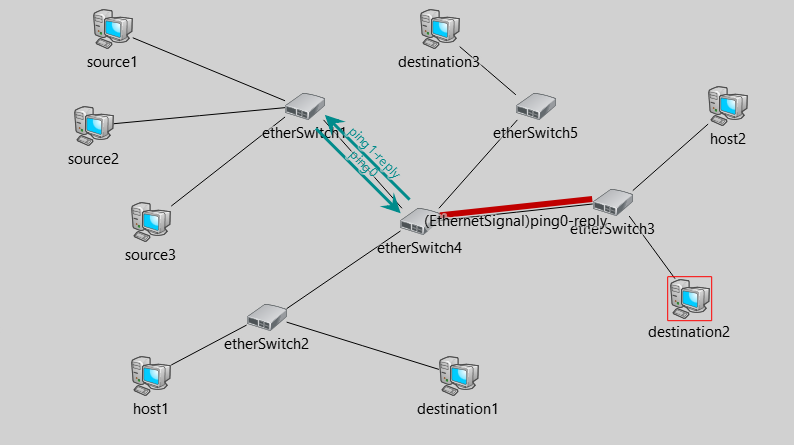
\includegraphics[width=\linewidth]{66}
			\end{minipage}\hfill
		\end{figure}
		
		\pagebreak
		
		\begin{figure}[!htb]
			\begin{minipage}{0.45\textwidth}
				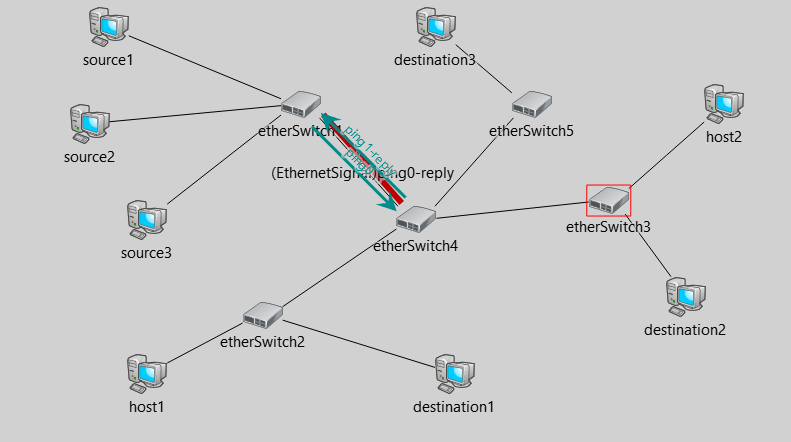
\includegraphics[width=\linewidth]{67}
			\end{minipage}\hfill
			\begin{minipage}{0.45\textwidth}
				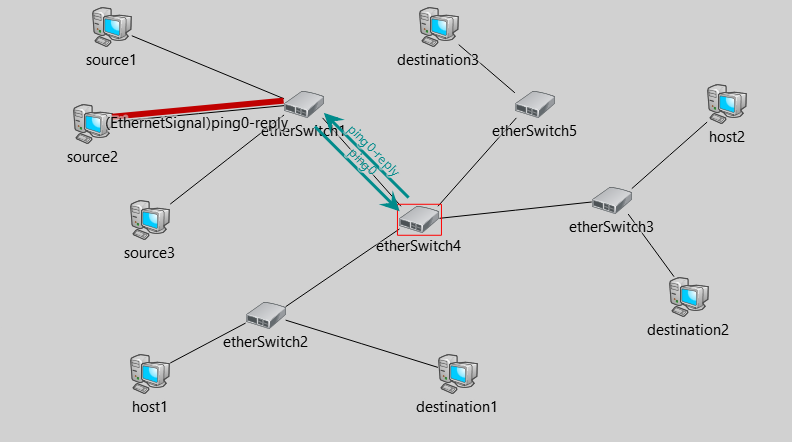
\includegraphics[width=\linewidth]{68}
			\end{minipage}\hfill
		\end{figure}
		\begin{figure}[!htb]
			\begin{minipage}{0.45\textwidth}
				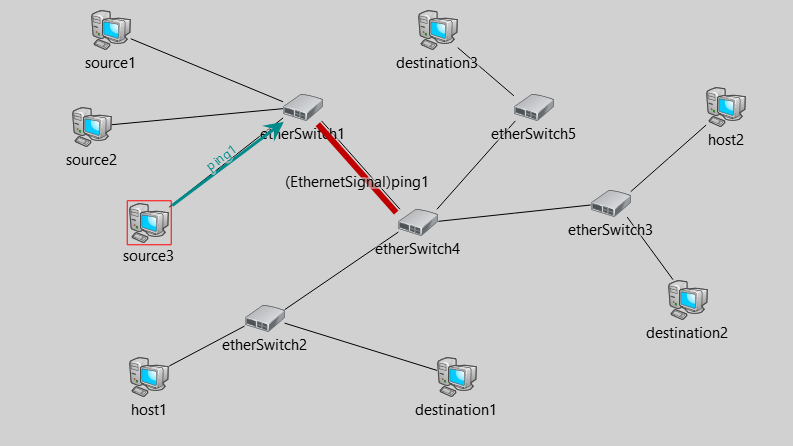
\includegraphics[width=\linewidth]{69}
			\end{minipage}\hfill
			\begin{minipage}{0.45\textwidth}
				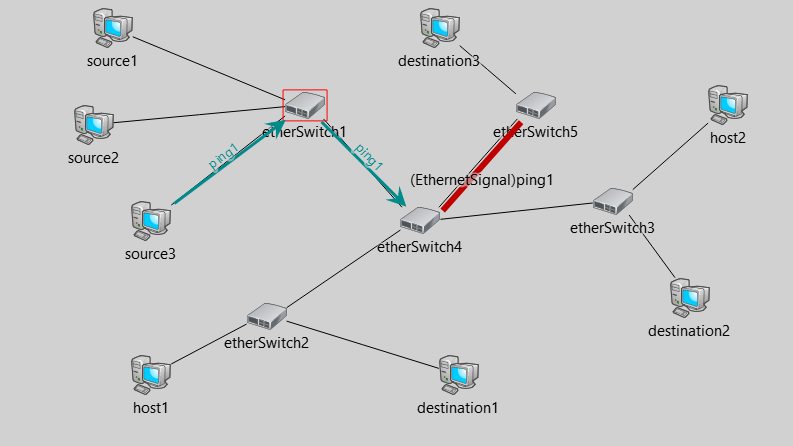
\includegraphics[width=\linewidth]{70}
			\end{minipage}\hfill
		\end{figure}
		\begin{figure}[!htb]
			\begin{minipage}{0.45\textwidth}
				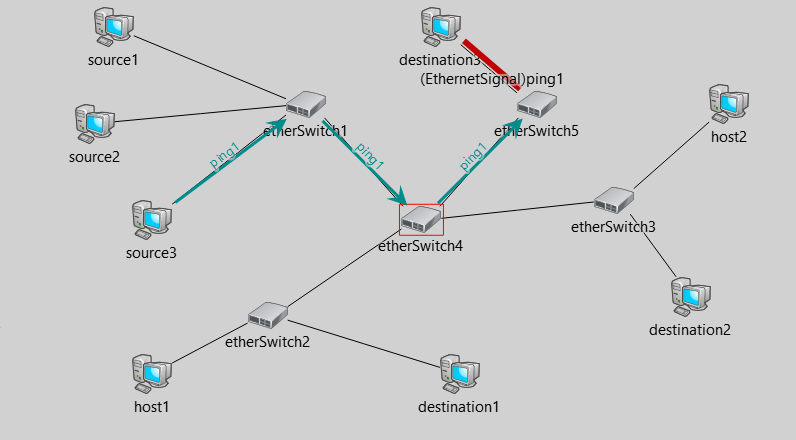
\includegraphics[width=\linewidth]{71}
			\end{minipage}\hfill
			\begin{minipage}{0.45\textwidth}
				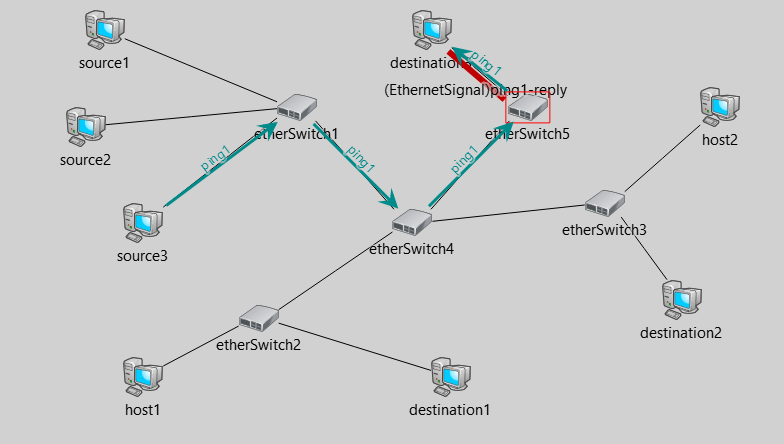
\includegraphics[width=\linewidth]{72}
			\end{minipage}\hfill
		\end{figure}
		\begin{figure}[!htb]
			\begin{minipage}{0.45\textwidth}
				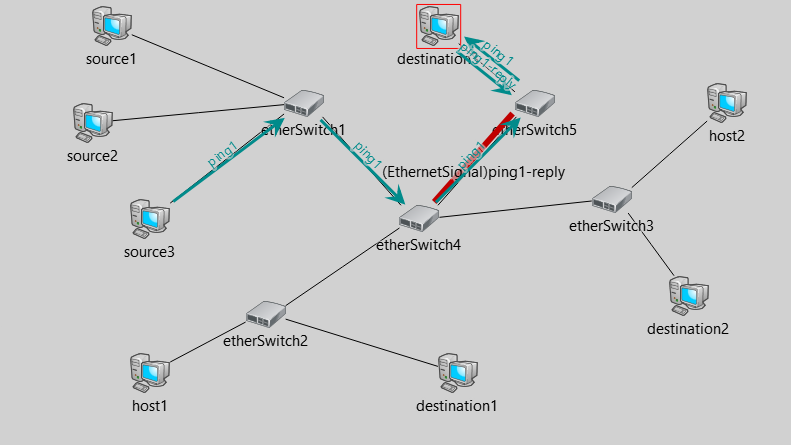
\includegraphics[width=\linewidth]{73}
			\end{minipage}\hfill
			\begin{minipage}{0.45\textwidth}
				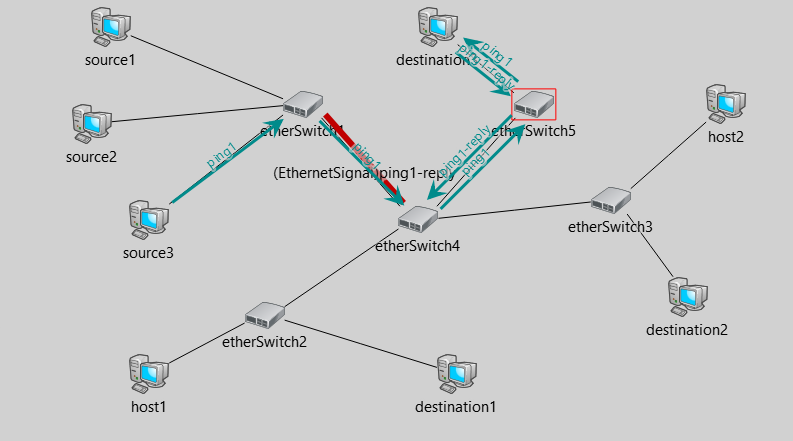
\includegraphics[width=\linewidth]{74}
			\end{minipage}\hfill
		\end{figure}
		\begin{figure}[!htb]
			\begin{minipage}{0.45\textwidth}
				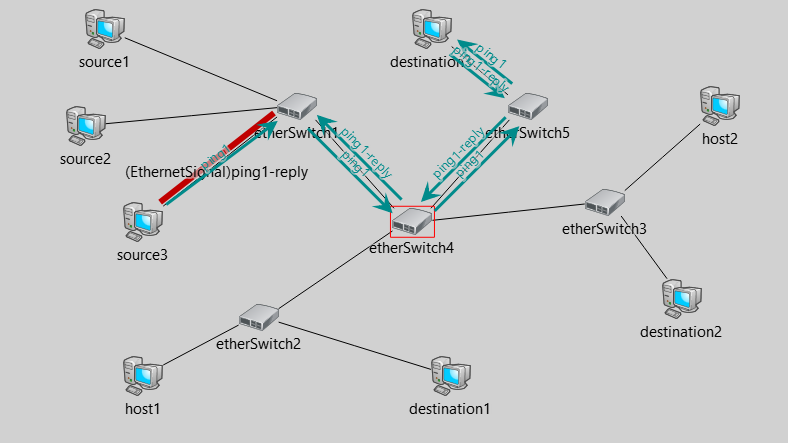
\includegraphics[width=\linewidth]{75}
			\end{minipage}\hfill
			\begin{minipage}{0.45\textwidth}
				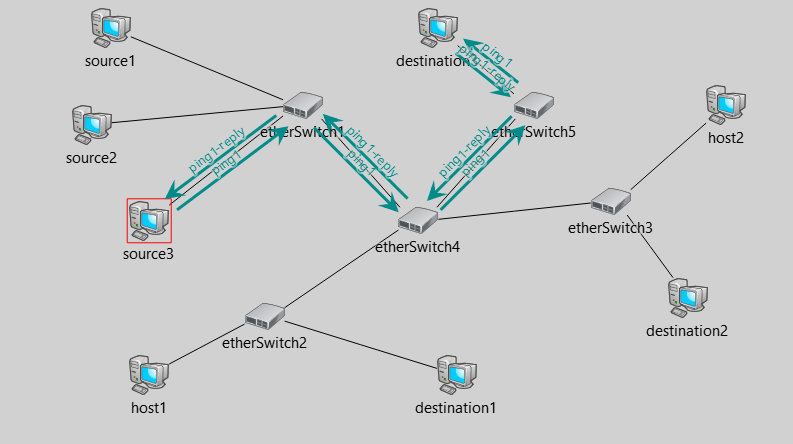
\includegraphics[width=\linewidth]{76}
			\end{minipage}\hfill
		\end{figure}
	\end{center}
	
	\pagebreak
	
	In this part, \textit{source3} first requests to send data to \textit{destination3} then it sends the ping data via ethernet switches 1, 4 and 5. And then \textit{destination3} sends the ping replies back to \textit{source3}. The arrows show the traffic path between the source and the destination.
	
	For this network data link activity visualization is filtered to display only ping messages.
	You can see that although there is both ARP and ping traffic in the network, DataLinkVisualizer only shows the ping messages as arrows, due to the presence of the packetFilter parameter.
	
	In this part I have used NodeFilter to display the traffic between \textit{source1} and \textit{destination1} along the path \textit{etherSwitch1}, \textit{etherSwitch4} and \textit{etherSwitch5}. As you observe, only the traffic in this path is displayed.
	
\end{document}